\chapter{AHTR One-Third Assembly Optimization Results}
\glsresetall
\label{chap:ahtr-assem-opt-results}
In this chapter, I report the \gls{AHTR} one-third assembly's \gls{ROLLO} optimization 
results. 
I vary the following \gls{AHTR} one-third assembly input parameters:
\begin{itemize}
    \item \gls{TRISO} packing fraction distribution ($\rho_{TRISO}(\vec{r})$)
    \item Total fuel packing fraction ($PF_{total}$)
    \item \gls{FLiBe} coolant channel shape
\end{itemize} 
And, I optimize the \gls{AHTR} one-third assembly for the following optimization 
objectives:
\begin{itemize}
    \item Minimize total fuel packing fraction ($PF_{total}$)
    \item Minimize maximum one-third assembly temperature ($T_{max}$)
    \item Minimize fuel-normalized power peaking factor ($PPF_{fuel}$)
\end{itemize} 
 
In Chapter \ref{chap:method}, I detailed the methodology for \gls{AHTR} one-third 
assembly modeling and \gls{ROLLO} optimization. 
Section \ref{sec:ahtr-assem-geometry} describes the \gls{AHTR} one-third assembly 
geometry.
Section \ref{sec:input-parameter-modeling} details about how I vary the 
\gls{AHTR} one-third assembly's input parameters. 
Sections \ref{sec:ahtr-moltres-hom} and \ref{sec:ahtr_model_verification}
describe and verify the \gls{AHTR} one-third assembly's OpenMC neutronics and Moltres 
temperature models. 
Section \ref{sec:opt-problem} describes the optimization objectives and Section 
\ref{sec:ahtr_slab_output} describes how I calculated them from the OpenMC and Moltres 
model outputs. 
Section \ref{sec:hyperparameter-studies} describes the hyperparameter tuning process 
to select hyperparameters for the single-objective and multi-objective \gls{ROLLO} 
optimization simulations.

The subsequent sections outline the \gls{AHTR} one-third assembly's optimization 
simulations, describe the results of the single-objective and multi-objective 
\gls{ROLLO} optimization simulations, report each simulation's computational cost, 
and discuss the results' significance.

\section{ROLLO AHTR One-Third Assembly Optimization Simulations Overview}
Table \ref{tab:assem-obj-breakdown} shows the details of each \gls{ROLLO} 
optimization problems explored in this chapter.
\begin{table}[htbp!]
    \centering
    \onehalfspacing
    \caption{\acrfull{ROLLO} simulations for optimizing \acrfull{AHTR}
    one-third assembly. $PF_{total}$: Total Fuel Packing Fraction, 
    $T_{max}$: Maximum one-third assembly Temperature, 
    $PPF_{fuel}$: Normalized Power Peaking Factor, $\rho_{TRISO}(\vec{r})$: 
    \gls{TRISO} packing fraction distribution}
	\label{tab:assem-obj-breakdown}
    \footnotesize
    \begin{tabular}{p{1.4cm}|p{1cm}|llll}
    \hline 
    \textbf{Num of Objs} & \textbf{Sim} & \textbf{Objectives} & \textbf{Constraints} &\textbf{Varying Parameters} & \textbf{Simulation Software} \\
    \hline
    \multirow{9}{2cm}{1}& a-1a & \tabitem min($PF_{total}$) & \tabitem $k_{eff}$ $>$ 1.38 &\tabitem $\rho_{TRISO}(\vec{r})$ & OpenMC \\
    & & & & \tabitem $PF_{total}$ & \\
    \cline{2-6}
    & a-1b & \tabitem min($T_{max}$) & \tabitem $k_{eff}$ $>$ 1.38 &\tabitem $\rho_{TRISO}(\vec{r})$ & OpenMC, Moltres\\
    \cline{2-6}
    & a-1c & \tabitem min($PPF_{fuel}$) & \tabitem $k_{eff}$ $>$ 1.38 &\tabitem $\rho_{TRISO}(\vec{r})$ & OpenMC\\
    \cline{2-6}
    & a-1d & \tabitem min($PF_{total}$) & \tabitem $k_{eff}$ $>$ 1.38 &\tabitem Coolant channel shape & OpenMC \\
    & & & & \tabitem $PF_{total}$ & \\
    \cline{2-6}
    & a-1e & \tabitem min($T_{max}$) & \tabitem $k_{eff}$ $>$ 1.38 &\tabitem Coolant channel shape & OpenMC, Moltres\\
    \cline{2-6}
    & a-1f & \tabitem min($PPF_{fuel}$) & \tabitem $k_{eff}$ $>$ 1.38 &\tabitem Coolant channel shape & OpenMC\\
    \hline
    \multirow{6}{2cm}{2}& a-2a & \tabitem min($PF_{total}$) & \tabitem $k_{eff}$ $>$ 1.38 & \tabitem $\rho_{TRISO}(\vec{r})$ & OpenMC, Moltres\\
    & &\tabitem min($T_{max}$) & & \tabitem $PF_{total}$ & \\
    \cline{2-6}
    & a-2b & \tabitem min($PF_{total}$) & \tabitem $k_{eff}$ $>$ 1.38 & \tabitem $\rho_{TRISO}(\vec{r})$ & OpenMC\\
    & & \tabitem min($PPF_{fuel}$) & & \tabitem $PF_{total}$ & \\
    \cline{2-6}
    & a-2c & \tabitem min($T_{max}$) & \tabitem $k_{eff}$ $>$ 1.38 & \tabitem $\rho_{TRISO}(\vec{r})$ & OpenMC, Moltres\\
    & & \tabitem min($PPF_{fuel}$) & & & \\
    \hline
    \multirow{6}{2cm}{3}& a-3a &\tabitem min($PF_{total}$) & \tabitem $k_{eff}$ $>$ 1.38 & \tabitem $\rho_{TRISO}(\vec{r})$ & OpenMC, Moltres\\
    && \tabitem min($PPF_{fuel}$) & & \tabitem $PF_{total}$ & \\
    && \tabitem min($T_{max}$) & & & \\
    \cline{2-6}
    & a-3b &\tabitem min($PF_{total}$) & \tabitem $k_{eff}$ $>$ 1.38 & \tabitem $\rho_{TRISO}(\vec{r})$ & OpenMC, Moltres\\
    && \tabitem min($PPF_{fuel}$) & & \tabitem $PF_{total}$ & \\
    && \tabitem min($T_{max}$) & & \tabitem Coolant channel shape& \\
    \hline
    \end{tabular}
\end{table}
I first conducted single objective, single input parameter \gls{ROLLO} optimizations 
to understand the individual impacts of each objective on each input parameter. 
Their results will inform the multi-objective optimization simulations setup. 
% TODO: update the keff constraint in table
% explain why some simulations use keff > 1.0 and that I didn't rerun because 
% I expect the same correlation results. 

Simulations are run on the Theta supercomputer at the Argonne Leadership Computing 
Facility under the Director's Discretionary Allocation Program 
\cite{noauthor_argonne_2022}. 
Section \ref{sec:assem-compute-cost} details each optimization simulation's computational 
cost.  

\section{AHTR One-Third Assembly: Single-Objective Optimization Results}
\label{sec:assem-one-obj}
This section reports the \gls{AHTR} one-third assembly's \gls{ROLLO} 
single-objective optimization results. 
Table \ref{tab:assem-obj-breakdown} summarized the one-objective simulations in this
section: a-1a, a-1b, a-1c, a-1d, a-1e, and a-1f. 
In the following subsections, I describe the single-objective optimization results 
grouped by the minimized objective. 

If a single-objective optimization problem's objective converges earlier than the 
5 generations I intended to run (determined in Section 
\ref{sec:multi-obj-hyperparameters}), I stop the simulation at that generation. 
Section \ref{sec:rollo-convergence} described how reactor designers use 
\gls{ROLLO} to determine problem convergence. 

\subsection{Objective: Minimize Total Packing Fraction ($PF_{total}$)}
\label{sec:assem-1-obj-pf}
This section reports the minimize total fuel packing fraction 
($PF_{total}$) single-objective optimization simulation results: a-1a and a-1d. 
Simulation a-1a varies the total fuel packing fraction ($PF_{total}$) and \gls{TRISO} 
packing fraction distribution ($\rho_{TRISO}(\vec{r})$), while simulation a-1d varies 
the total fuel packing fraction ($PF_{total}$) and coolant channel shape. 

\subsubsection{Simulation a-1a: Variation of $\rho_{TRISO}(\vec{r})$ and $PF_{total}$}
Table \ref{tab:simulationa1a} shows simulation a-1a's optimization problem parameters. 
\begin{table}[htbp!]
    \centering
    \onehalfspacing
    \caption{Simulation a-1a Optimization Problem Parameters}
	\label{tab:simulationa1a}
    \footnotesize
    \begin{tabular}{l|p{5.3cm}}
    \hline 
    \multicolumn{2}{c}{\textbf{Single Objective: Simulation a-1a}} \\
    \hline 
    \textbf{Objectives} & Minimize $PF_{total}$ \\
    \hline 
    \textbf{Input Parameter Variations} & $0.05<PF_{total}<0.07$ \\
    & $\rho_{TRISO}(\vec{r})$: $0<a<2$, $0<d<2$\\
    & $\rho_{TRISO}(\vec{r})$: $0<b<\frac{\pi}{2}$, $0<e<\frac{\pi}{2}$\\
    & $\rho_{TRISO}(\vec{r})$: $0<c<2\pi$, $0<f<2\pi$\\
    \hline
    \textbf{Constraints} & $k_{eff} \geq 1.38$\\ 
    \hline 
    \textbf{Genetic Algorithm Parameters} & Population size: 128 \\
    & Generations: 3 \\
    \hline
    \end{tabular}
\end{table}

Figure \ref{fig:assem-obj-1-pf-evol} shows the $PF_{total}$ evolution.
Figure \ref{fig:assem-obj-1-pf-final} shows four unique TRISO packing fraction distributions 
in the final generation with the most-minimized $PF_{total}$. 
Figure \ref{fig:assem-obj-1-pf-most-minimized} illustrates the \gls{AHTR} one-third 
assembly model with the most-minimized $PF_{total}$.
\begin{figure}[htbp!]
    \begin{subfigure}{\textwidth}
        \centering
        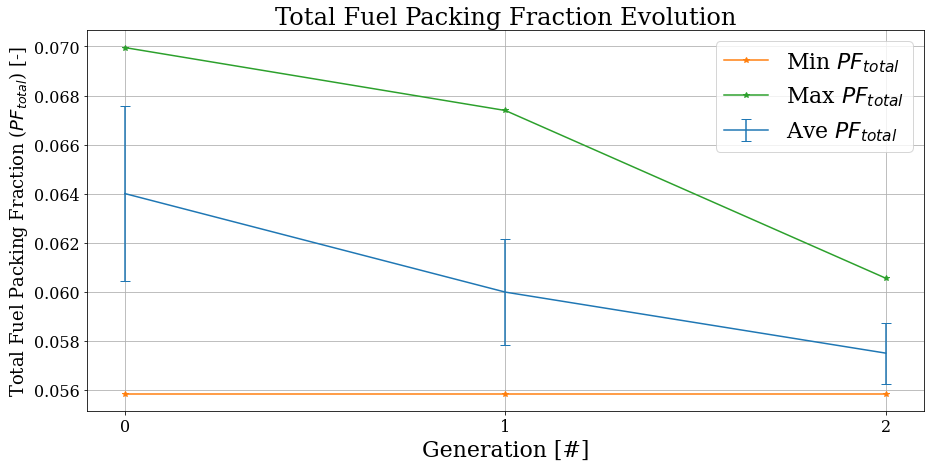
\includegraphics[width=\linewidth]{assem-obj-1-pf-evol.png}
        \caption{Minimum, average, and maximum $PF_{total}$ evolution.}
        \label{fig:assem-obj-1-pf-evol} 
    \end{subfigure}
    \begin{subfigure}{\textwidth}
        \centering
        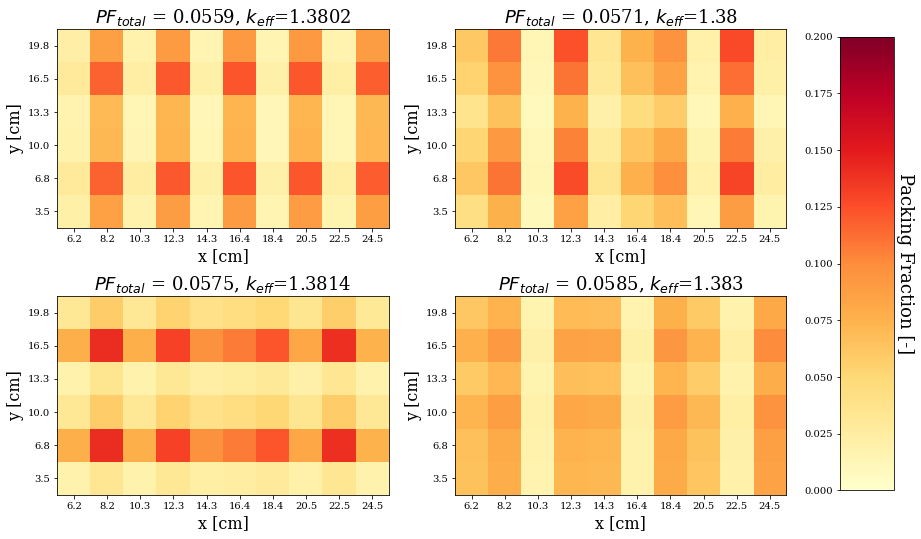
\includegraphics[width=\linewidth]{assem-obj-1-pf-final.png}
        \caption{TRISO packing fraction distribution for four unique reactor models with the 
        smallest $PF_{total}$ in the final generation.}
        \label{fig:assem-obj-1-pf-final} 
    \end{subfigure}
    \caption{Simulation a-1a -- ROLLO single-objective optimization to minimize total 
    fuel packing fraction ($PF_{total}$) in \gls{AHTR} one-third assembly. 
    Input parameters varied: total fuel packing fraction 
    ($PF_{total}$), \gls{TRISO} packing fraction distribution ($\rho_{TRISO}(\vec{r})$).}
    \label{fig:assem-obj-1-pf}
\end{figure}
\begin{figure}[htbp!]
    \ContinuedFloat
    \begin{subfigure}{\textwidth}
        \centering
        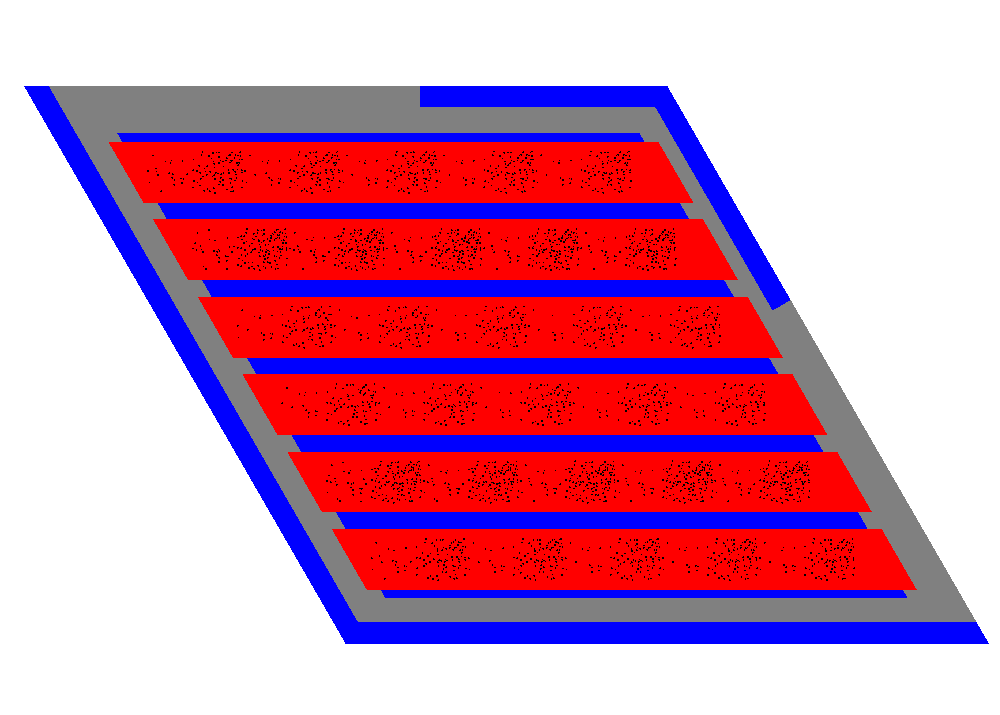
\includegraphics[width=0.7\linewidth]{assem-obj-1-pf-most-minimized.png}
        \caption{\gls{AHTR} one-third assembly model with the most-minimized 
        $PF_{total}$, corresponding to the the first TRISO distribution in Figure 
        \ref{fig:assem-obj-1-pf-final}. The reactor model has $PF_{total}=0.0559$
        and $k_{eff}=1.3802$.}
        \label{fig:assem-obj-1-pf-most-minimized} 
    \end{subfigure}
    \caption{(contd.) Simulation a-1a -- ROLLO single-objective optimization to minimize total 
    fuel packing fraction ($PF_{total}$) in \gls{AHTR} one-third assembly. 
    Input parameters varied: total fuel packing fraction 
    ($PF_{total}$), \gls{TRISO} packing fraction distribution ($\rho_{TRISO}(\vec{r})$).}
\end{figure}

Figure \ref{fig:assem-obj-1-pf-evol} shows that the minimum and average $PF_{total}$ 
converged quickly, as expected in this single-objective optimization problem.
By the final generation, the average and minimum $PF_{total}$
values converged to approximately 0.057. 
In Figure \ref{fig:assem-obj-1-pf-final}, the four unique TRISO packing fraction 
distributions in the final generation that most-minimized $PF_{total}$ have various 
oscillating TRISO distribution patterns. 

The one-third assembly model with the most-minimized $PF_{total}$ has a 
$PF_{total} =0.0559$ and an oscillating TRISO distribution along the both the 
x-axis and y-axis, and a packing fraction standard deviation of $0.04$ across the 
one-third assembly. 
Along the x-axis, the distribution peaks on the even fuel cell columns (at 8.2cm, 12.3cm, 
16.4cm, 20.5cm, and 24.5cm). 
The even columns have the largest y-axis variation of $\sim0.05$ with peaks of
$PF\approx0.12$.
The odd columns have the smallest y-axis variation of $\sim0.01$ with minimums of 
$PF\approx0.012$.
Along the y-axis, the distribution peaks on the 2nd and 5th fuel cell rows (at 6.8cm and 
16.5cm).
The 2nd and 5th row have the largest x-axis variation of $\sim0.10$ and the middle 3rd 
and 4th rows have the smallest x-axis variation of $\sim0.06$.

Section \ref{sec:assem-discussion-pf} discusses the driving factors for the minimize 
$PF_{total}$ objective and explains simulation a-1a's most-minimized $PF_{total}$ 
oscillating TRISO distribution. 

\subsubsection{Simulation a-1d: Variation of $PF_{total}$ and Coolant channel shape}
Table \ref{tab:simulationa1d} shows simulation a-1d's optimization problem parameters. 
\begin{table}[htbp!]
    \centering
    \onehalfspacing
    \caption{Simulation a-1d Optimization Problem Parameters}
	\label{tab:simulationa1d}
    \footnotesize
    \begin{tabular}{l|p{6cm}}
    \hline 
    \multicolumn{2}{c}{\textbf{Single Objective: Simulation a-1d}} \\
    \hline 
    \textbf{Objectives} & Minimize $PF_{total}$ \\
    \hline 
    \textbf{Input Parameter variations} & $0.01<PF_{total}<0.04$ \\
    & coolant channel shape: $0.05<r_{1}<0.35$ \\
    & coolant channel shape: $0.05<r_{2}<0.35$ \\
    & coolant channel shape: $0.05<r_{3}<0.35$ \\
    & coolant channel shape: $0.05<r_{4}<0.35$ \\
    & coolant channel shape: $0.05<r_{5}<0.35$ \\
    \hline
    \textbf{Constraints} & $k_{eff} \geq 1.0$\\ 
    \hline 
    \textbf{Genetic Algorithm Parameters} & Population size: 64 \\
    & Generations: 2 \\
    \hline
    \end{tabular}
\end{table}

Figure \ref{fig:a-1d} shows the plots of coolant channel shape's 
$r_1, r_2, r_3, r_4,$ and $r_5$ values against $PF_{total}$. 
\begin{figure}[htbp!]
    \centering
    \begin{subfigure}{0.49\textwidth}
        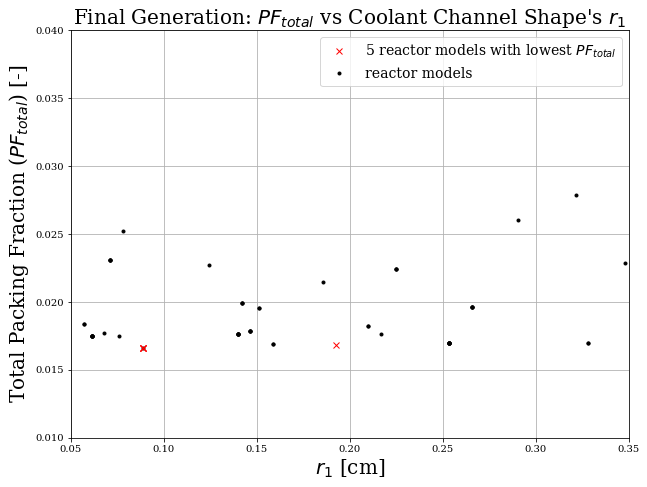
\includegraphics[width=\linewidth]{a-1d-r1.png}
        \caption{Plot of $PF_{total}$ against $r_1$.}
        \label{fig:a-1d-r1} 
    \end{subfigure}
    \begin{subfigure}{0.49\textwidth}
        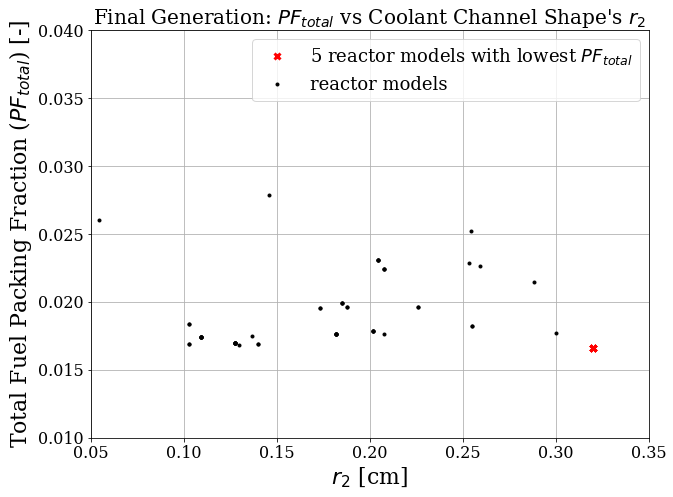
\includegraphics[width=\linewidth]{a-1d-r2.png}
        \caption{Plot of $PF_{total}$ against $r_2$.}
        \label{fig:a-1d-r2} 
    \end{subfigure}
    \begin{subfigure}{0.49\textwidth}
        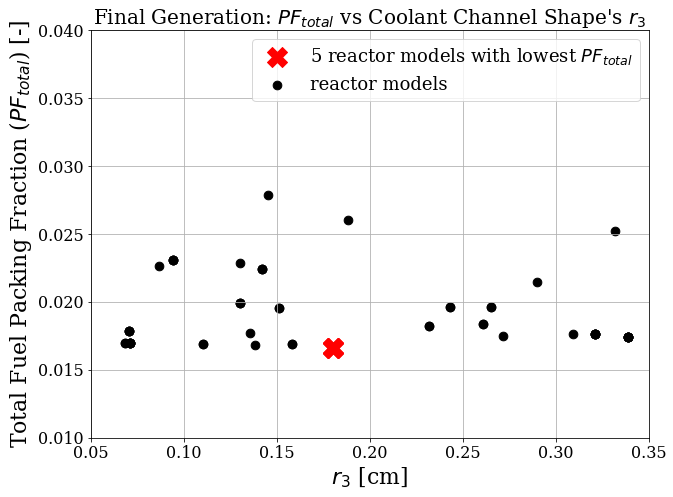
\includegraphics[width=\linewidth]{a-1d-r3.png}
        \caption{Plot of $PF_{total}$ against $r_3$.}
        \label{fig:a-1d-r3} 
    \end{subfigure}
    \begin{subfigure}{0.49\textwidth}
        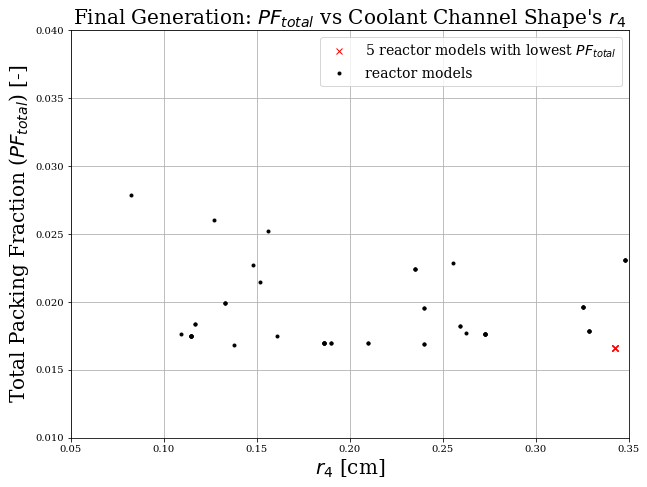
\includegraphics[width=\linewidth]{a-1d-r4.png}
        \caption{Plot of $PF_{total}$ against $r_4$.}
        \label{fig:a-1d-r4} 
    \end{subfigure}
    \begin{subfigure}{0.49\textwidth}
        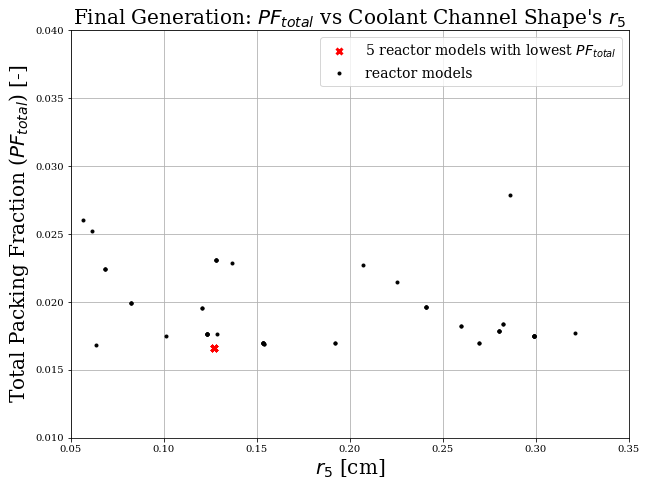
\includegraphics[width=\linewidth]{a-1d-r5.png}
        \caption{Plot of $PF_{total}$ against $r_5$.}
        \label{fig:a-1d-r5} 
    \end{subfigure}
    \caption{Simulation a-1d -- ROLLO single-objective optimization to minimize 
    total fuel packing fraction($PF_{total}$). 
    Plots of simulation a-1d final generation's reactor models $PF_{total}$ against 
    coolant channel shape input parameters. 
    Red crosses indicate the five reactor models with the lowest $PF_{total}$.
    Input parameters varied: total fuel packing fraction 
    ($PF_{total}$), and coolant channel shape ($r_1, r_2, r_3, r_4, r_5$).}
    \label{fig:a-1d}
\end{figure}

Figure \ref{fig:a-1d} demonstrates that there is no correlation between $PF_{total}$ 
and coolant channel shape's $r_1, r_2, r_3, r_4,$ and $r_5$. 

\subsection{Objective: Minimize Maximum Temperature ($T_{max}$)}
\label{sec:assem-1-obj-temp}
This section reports results from the minimize maximum one-third assembly temperature 
($T_{max}$) single-objective optimization simulations: a-1b and a-1e. 
Simulation a-1b varies \gls{TRISO} packing fraction distribution 
($\rho_{TRISO}(\vec{r})$), while simulation a-1e varies the coolant channel shape. 

\subsubsection{Simulation a-1b: Variation of $\rho_{TRISO}(\vec{r})$}
Table \ref{tab:simulationa1b} shows simulation a-1b's optimization problem parameters. 
\begin{table}[htbp!]
    \centering
    \onehalfspacing
    \caption{Simulation a-1b Optimization Problem Parameters}
	\label{tab:simulationa1b}
    \footnotesize
    \begin{tabular}{l|p{5.3cm}}
    \hline 
    \multicolumn{2}{c}{\textbf{Single Objective: Simulation a-1b}} \\
    \hline 
    \textbf{Objectives} & Minimize $T_{max}$ \\
    \hline 
    \textbf{Input Parameter variations} 
    & $\rho_{TRISO}(\vec{r})$: $0<a<2$, $0<d<2$\\
    & $\rho_{TRISO}(\vec{r})$: $0<b<\frac{\pi}{2}$, $0<e<\frac{\pi}{2}$\\
    & $\rho_{TRISO}(\vec{r})$: $0<c<2\pi$, $0<f<2\pi$\\
    \hline
    \textbf{Constraints} & $k_{eff} \geq 1.0$\\ 
    & $PF_{total} = 0.04 $\\ 
    \hline 
    \textbf{Genetic Algorithm Parameters} & Population size: 64 \\
    & Generations: 3 \\
    \hline
    \end{tabular}
\end{table}

The TRISO distribution is varied based on sine distributions, as described 
in Section \ref{sec:input-parameter-modeling}. 
If the simulation used the FHR benchmark equivalent $PF_{total} = 0.153$, at
certain sine distributions, some fuel cells will have $PF > 0.3$. 
OpenMC's random sequential packing algorithm becomes prohibitively slow at $PF > 0.3$, 
resulting in long runtimes. 
Therefore, I used $PF_{total} = 0.06$ because it is approximately the smallest 
$PF_{total}$ that enables $k_{eff} \geq 1.38$ and will avoid fuel cells with 
$PF > 0.3$ occurences. 
I use $PF_{total} = 0.06$ for all optimization simulations that do not vary 
$PF_{total}$: a-1c, a-1e, a-1f, a-2c. 

Figure \ref{fig:assem-obj-1-temp-evol} shows the one-third assembly's $T_{max}$ 
evolution. 
Figure \ref{fig:assem-obj-1-temp-final} shows four unique TRISO packing fraction 
distributions in the final generation with the most minimized $T_{max}$. 
Figure \ref{fig:assem-obj-1-temp-most-minimized} illustrates the \gls{AHTR} one-third 
assembly model with the most-minimized $T_{max}$. 
\begin{figure}[htbp!]
    \begin{subfigure}{\textwidth}
        \centering
        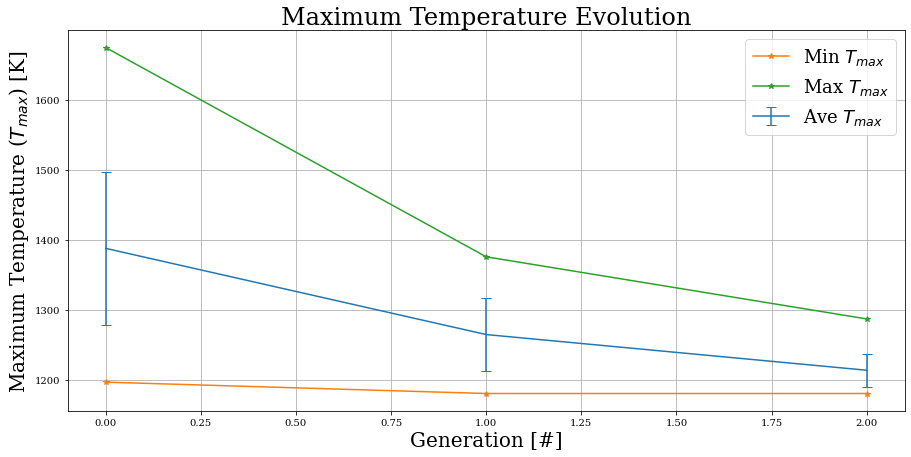
\includegraphics[width=\linewidth]{assem-obj-1-temp-evol.png}
        \caption{Minimum, average, and maximum $T_{max}$ evolution.}
        \label{fig:assem-obj-1-temp-evol} 
    \end{subfigure}
    \begin{subfigure}{\textwidth}
        \centering
        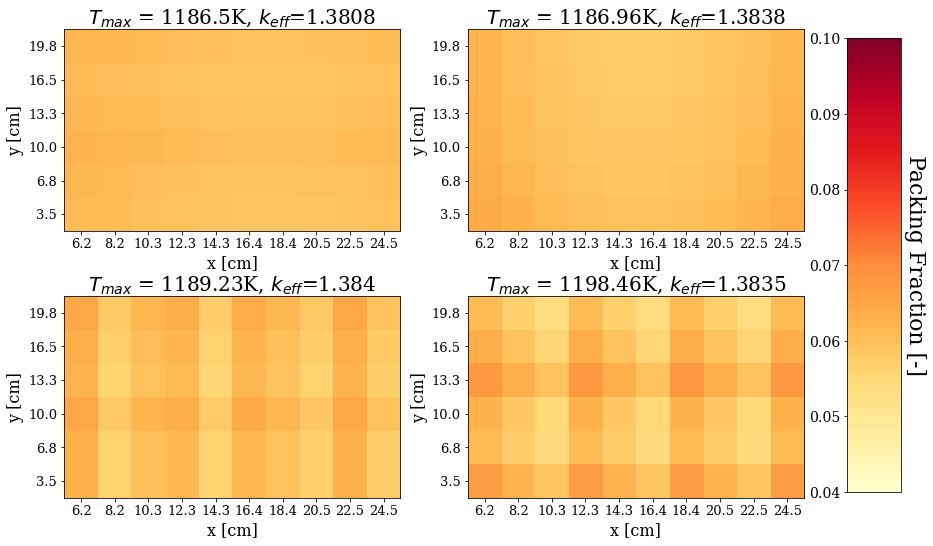
\includegraphics[width=\linewidth]{assem-obj-1-temp-final.png}
        \caption{TRISO packing fraction distribution for four unique reactor models with the 
        smallest $T_{max}$ in the final generation.}
        \label{fig:assem-obj-1-temp-final} 
    \end{subfigure}
    \caption{Simulation a-1b -- ROLLO single-objective optimization to minimize maximum 
    temperature ($T_{max}$) in \gls{AHTR} one-third assembly. 
    Input parameters varied: \gls{TRISO} packing fraction distribution 
    ($\rho_{TRISO}(\vec{r})$).}
    \label{fig:assem-obj-1-temp}
\end{figure}
\begin{figure}[htbp!]
    \ContinuedFloat
    \begin{subfigure}{\textwidth}
        \centering
        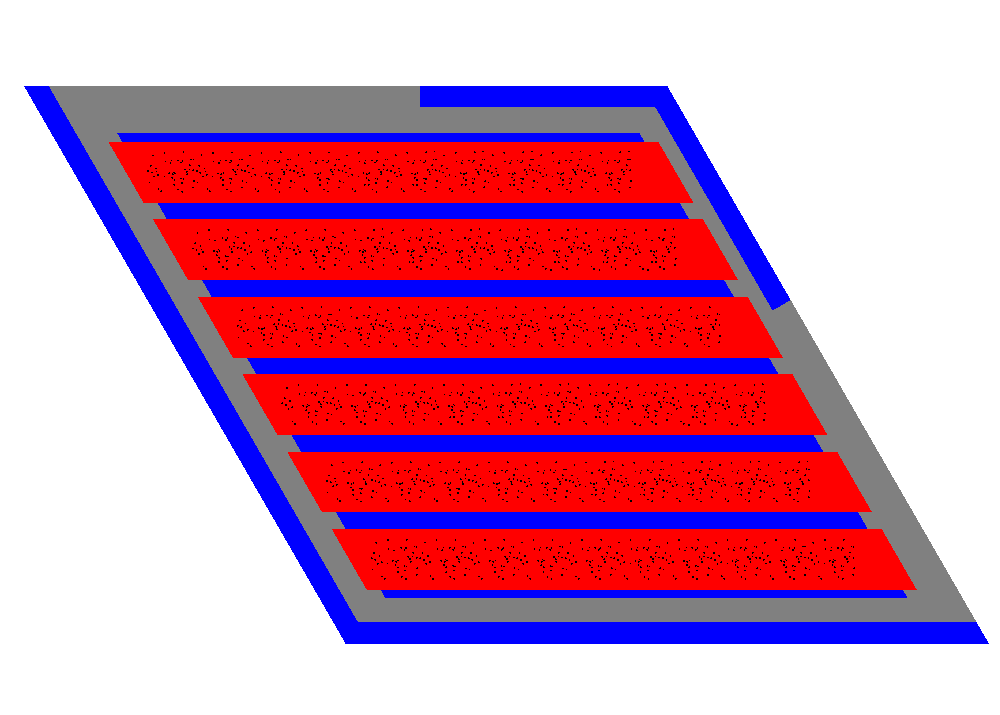
\includegraphics[width=0.7\linewidth]{assem-obj-1-temp-most-minimized.png}
        \caption{\gls{AHTR} one-third assembly model with the most-minimized 
        $T_{max}$, corresponding to the the first TRISO distribution in Figure 
        \ref{fig:assem-obj-1-temp-final}. The reactor model has $T_{max}=1180.29$K
        and $k_{eff}=1.3046$.}
        \label{fig:assem-obj-1-temp-most-minimized} 
    \end{subfigure}
    \caption{Simulation a-1b -- ROLLO single-objective optimization to minimize maximum 
    temperature ($T_{max}$) in \gls{AHTR} one-third assembly. 
    Input parameters varied: \gls{TRISO} packing fraction distribution 
    ($\rho_{TRISO}(\vec{r})$).}
\end{figure}

Figure \ref{fig:assem-obj-1-temp-evol} shows that the minimum and average one-third 
assembly's $T_{max}$ converged to approximately 1200 K.
In Figure \ref{fig:assem-obj-1-temp-final}, the one-third assembly model with the 
most-minimized $T_{max}$ has a $T_{max}=1180.3$K and an almost constant TRISO packing 
fraction distribution.
% TODO: update with new results

\subsubsection{Simulation a-1e: Variation of Coolant channel shape}
Table \ref{tab:simulationa1e} shows simulation a-1e's optimization problem parameters. 
\begin{table}[htbp!]
    \centering
    \onehalfspacing
    \caption{Simulation a-1e Optimization Problem Parameters}
	\label{tab:simulationa1e}
    \footnotesize
    \begin{tabular}{l|p{6cm}}
    \hline 
    \multicolumn{2}{c}{\textbf{Single Objective: Simulation a-1e}} \\
    \hline 
    \textbf{Objectives} & Minimize $T_{max}$ \\
    \hline 
    \textbf{Input Parameter variations} 
    & coolant channel shape: $0.05<r_{1}<0.35$ \\
    & coolant channel shape: $0.05<r_{2}<0.35$ \\
    & coolant channel shape: $0.05<r_{3}<0.35$ \\
    & coolant channel shape: $0.05<r_{4}<0.35$ \\
    & coolant channel shape: $0.05<r_{5}<0.35$ \\
    \hline
    \textbf{Constraints} & $k_{eff} \geq 1.0$\\ 
    & $PF_{total} = 0.04 $\\ 
    \hline 
    \textbf{Genetic Algorithm Parameters} & Population size: 64 \\
    & Generations: 3 \\
    \hline
    \end{tabular}
\end{table}

Figure \ref{fig:a-1e-evol} shows the one-third assembly's $T_{max}$ evolution.
Figure \ref{fig:assem-obj-1-temp-most-minimized-coolant} illustrates the \gls{AHTR} 
one-third assembly model with the most-minimized $T_{max}$. 
Figures \ref{fig:a-1e-r1}, \ref{fig:a-1e-r2}, \ref{fig:a-1e-r3}, \ref{fig:a-1e-r4}, 
and \ref{fig:a-1e-r5} show the plots of coolant channel shape's 
$r_1, r_2, r_3, r_4,$ and $r_5$ values against $T_{max}$. 
\begin{figure}[htbp!]
    \begin{subfigure}{\textwidth}
        \centering
        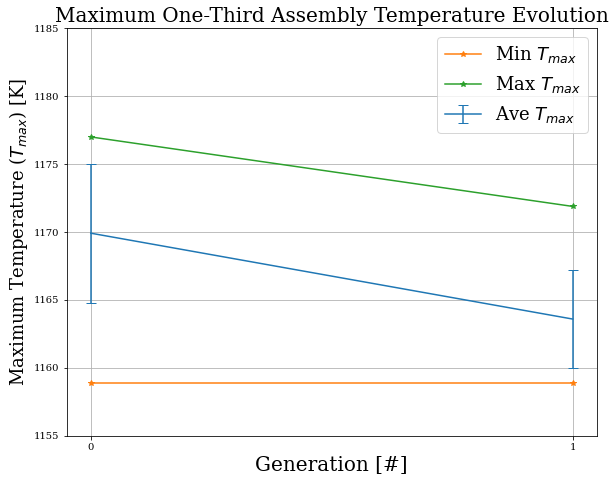
\includegraphics[width=\linewidth]{a-1e-evol.png}
        \caption{Minimum, average, and maximum evolution of AHTR one-third assembly's 
        $T_{max}$.}
        \label{fig:a-1e-evol} 
    \end{subfigure}
    \begin{subfigure}{\textwidth}
        \centering
        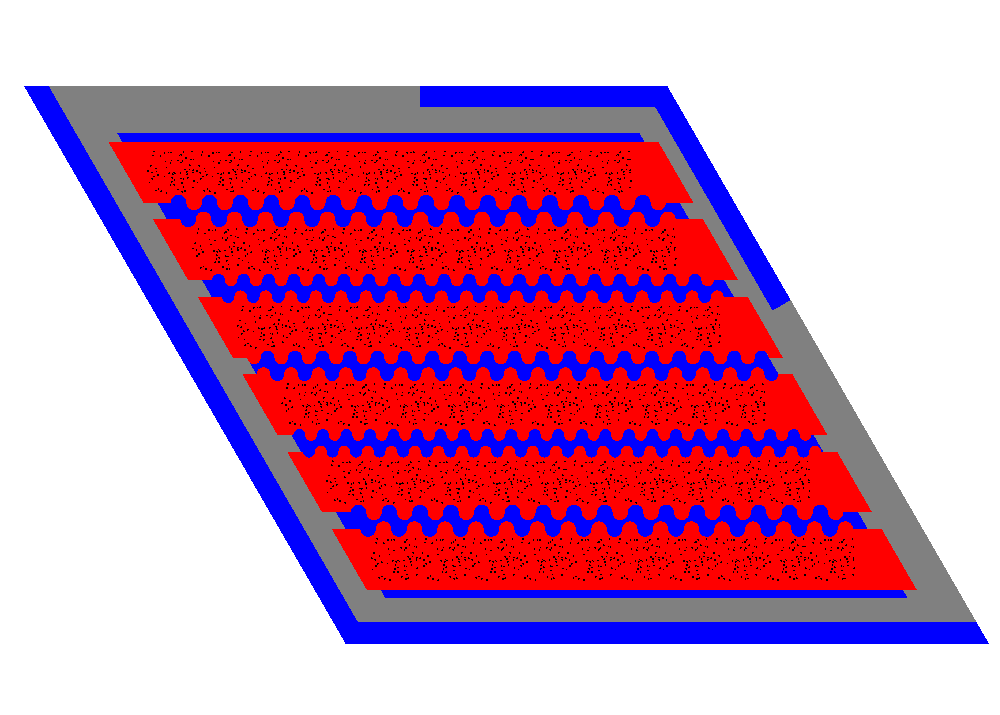
\includegraphics[width=0.8\linewidth]{assem-obj-1-temp-most-minimized-coolant.png}
        \caption{\gls{AHTR} one-third assembly model with the most-minimized $T_{max}$. 
        The reactor model has $T_{max} = 1158.39K$, $r_1 = 0.33cm$, $r_{2} = 0.19cm$,
        $r_3 = 0.22cm$, $r_{4} = 0.21cm$, and $r_{5} = 0.32cm$.}
        \label{fig:assem-obj-1-temp-most-minimized-coolant} 
    \end{subfigure}
    \caption{Simulation a-1e -- ROLLO single-objective optimization to minimize 
    maximum one-third assembly temperature ($T_{max}$). 
    Plots of final generation's reactor models $T_{max}$ against 
    coolant channel shape input parameters. 
    Red crosses indicate the five reactor models with the lowest $T_{max}$.
    Input parameters varied: coolant channel shape ($r_1, r_2, r_3, r_4, r_5$).}
    \label{fig:a-1e}
\end{figure}
\begin{figure}[htbp!]
    \ContinuedFloat
    \centering
    \begin{subfigure}{0.49\textwidth}
        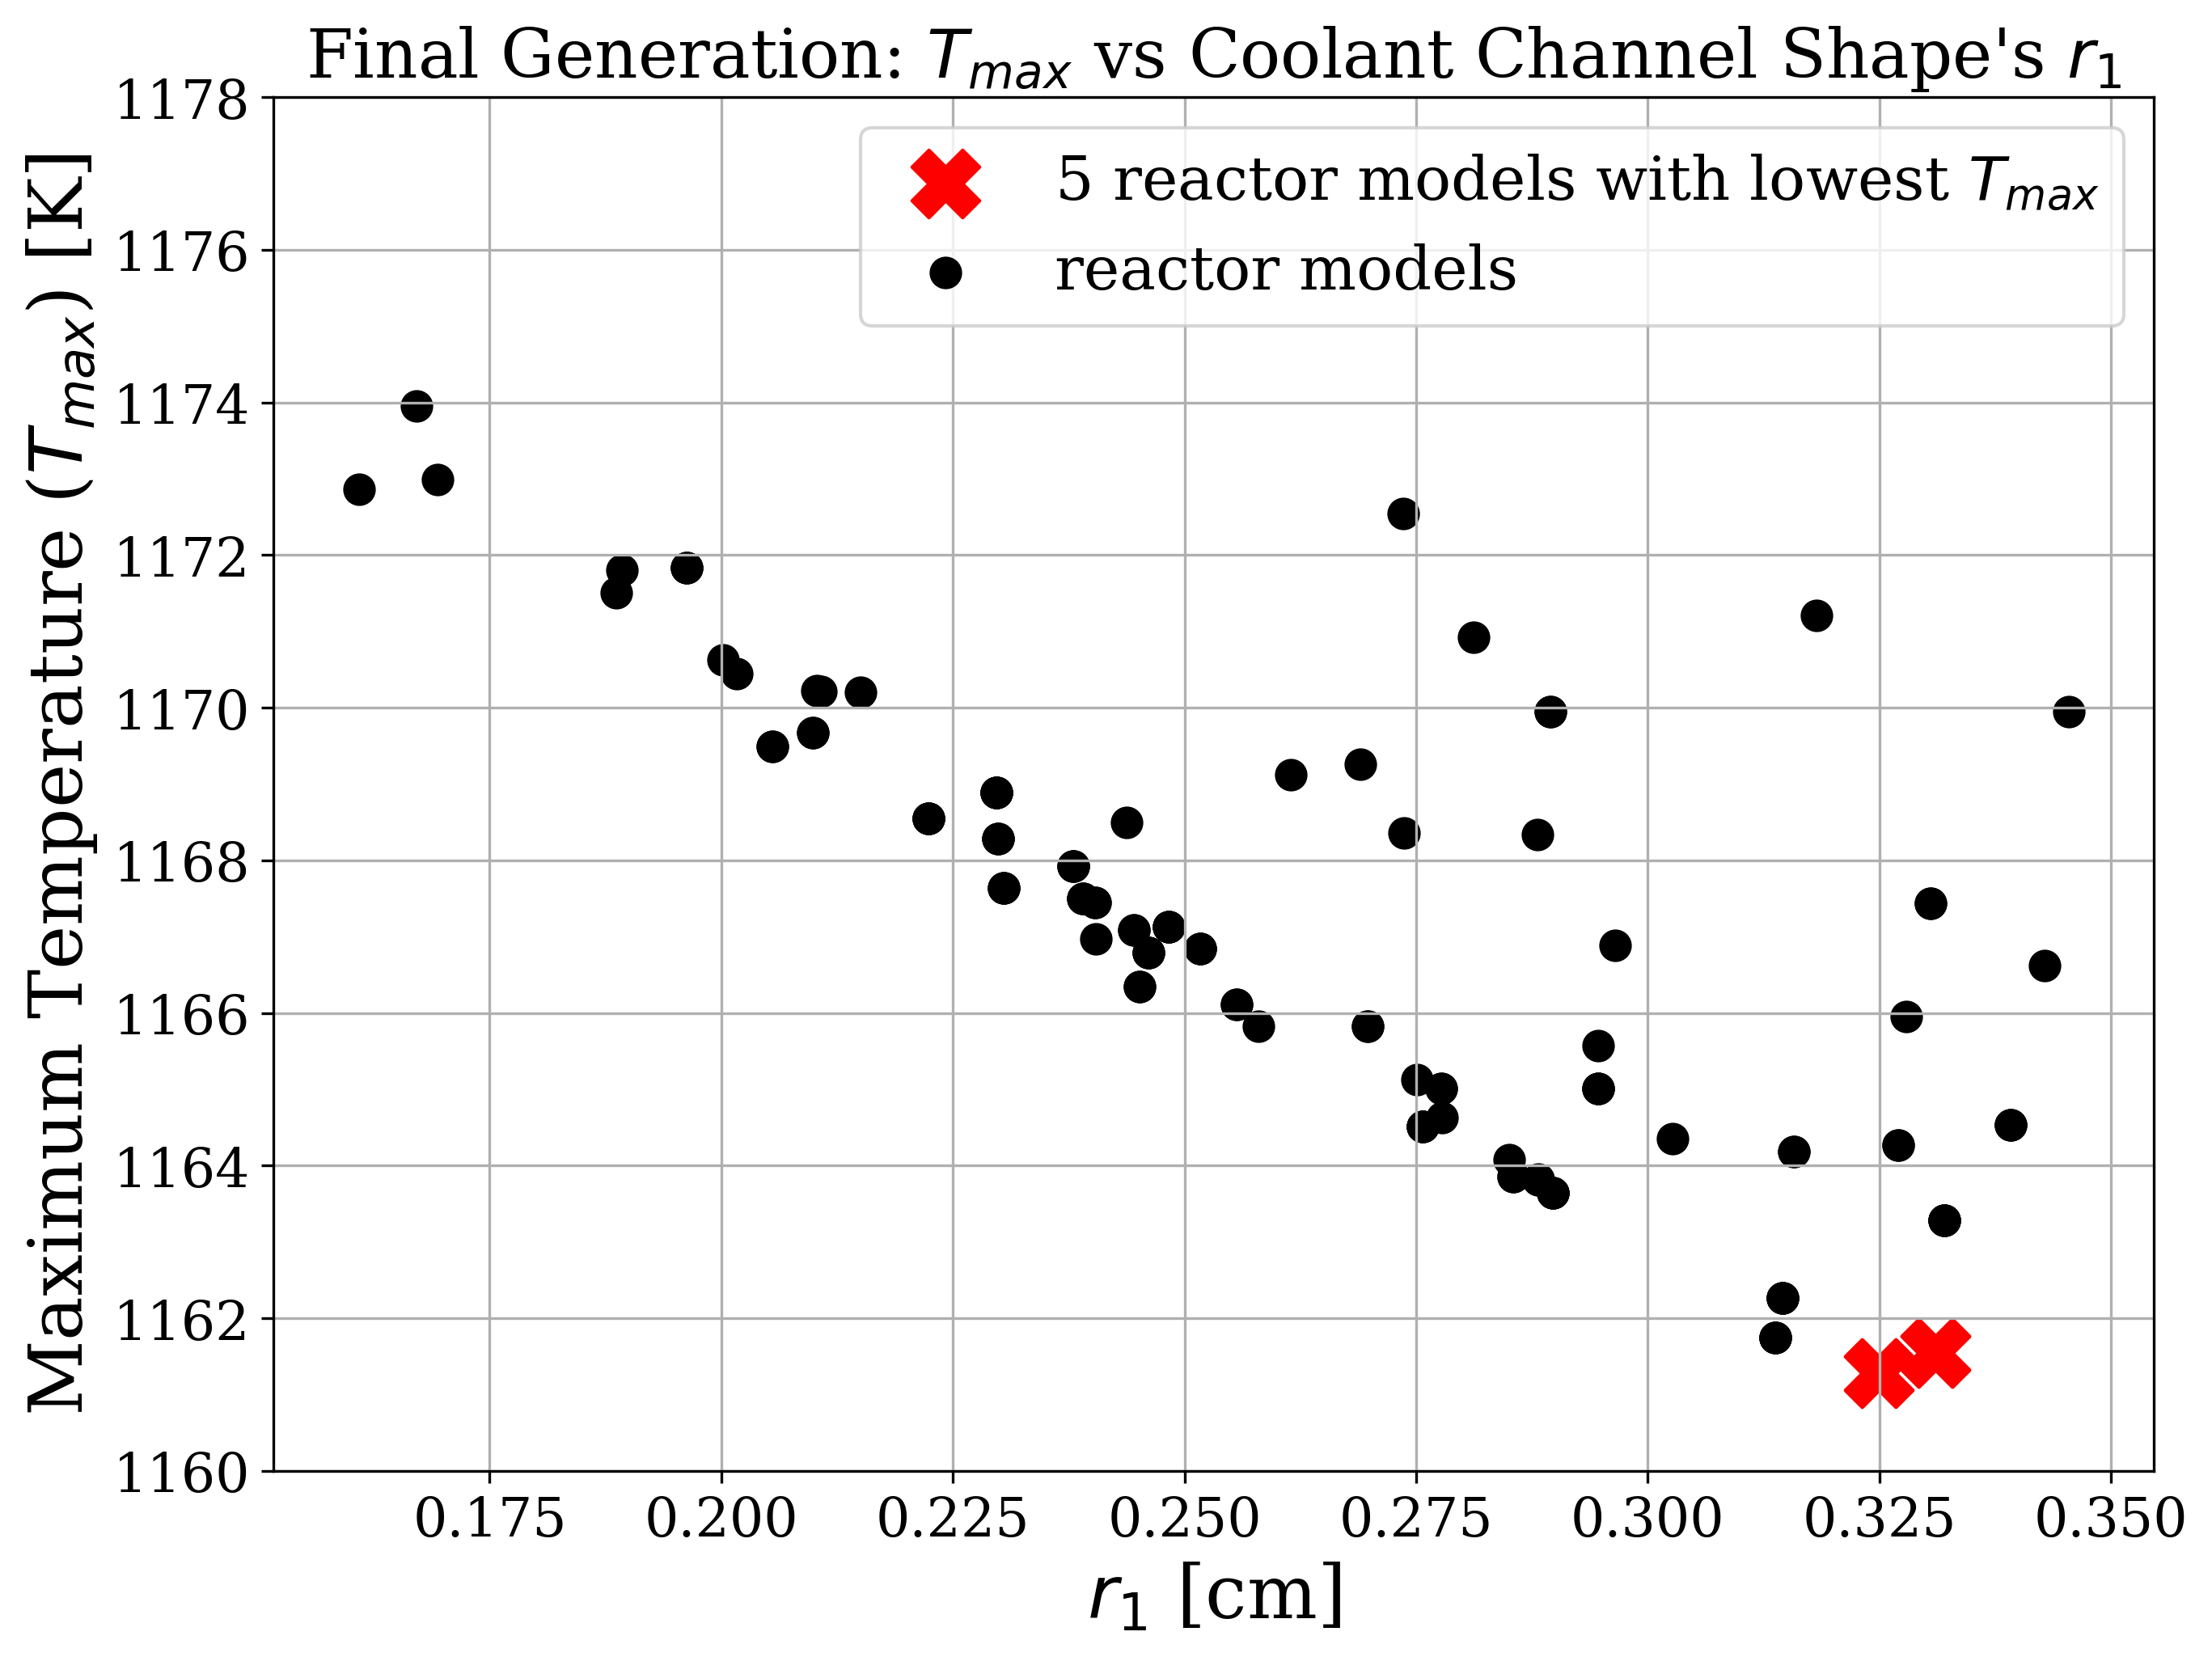
\includegraphics[width=\linewidth]{a-1e-r1.png}
        \caption{Plot of $PF_{total}$ against $r_1$.}
        \label{fig:a-1e-r1} 
    \end{subfigure}
    \begin{subfigure}{0.49\textwidth}
        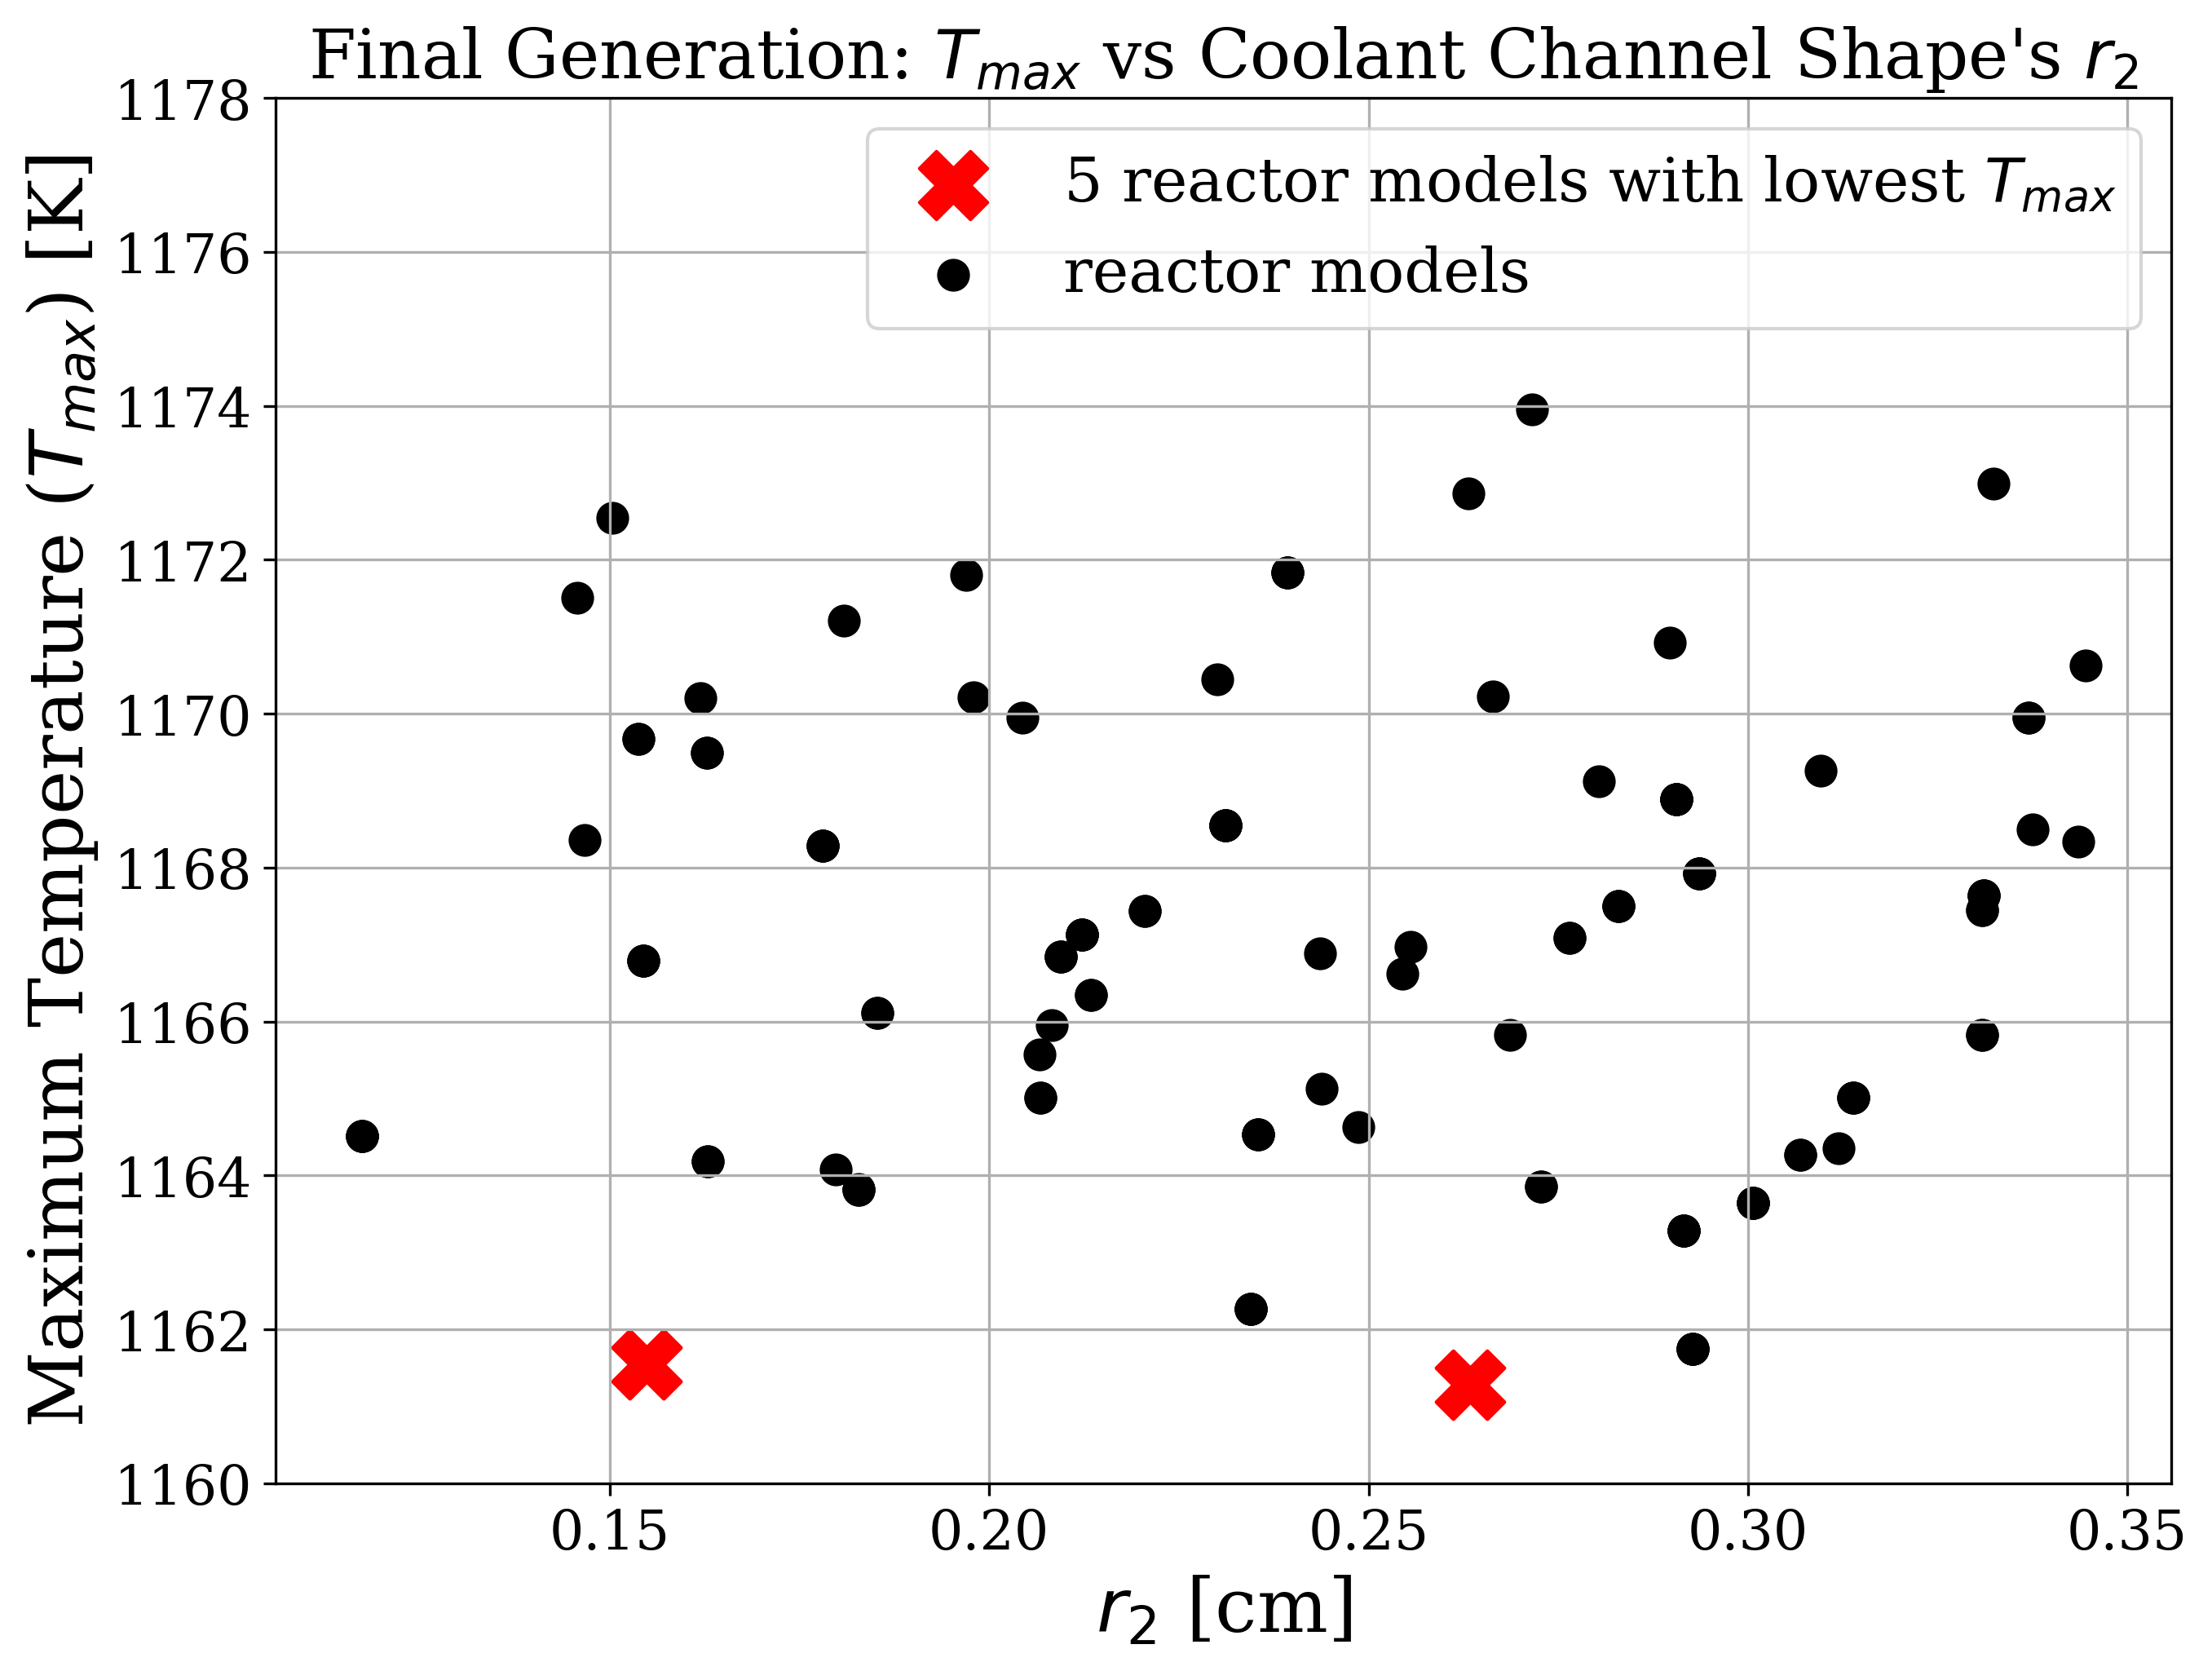
\includegraphics[width=\linewidth]{a-1e-r2.png}
        \caption{Plot of $PF_{total}$ against $r_2$.}
        \label{fig:a-1e-r2} 
    \end{subfigure}
    \begin{subfigure}{0.49\textwidth}
        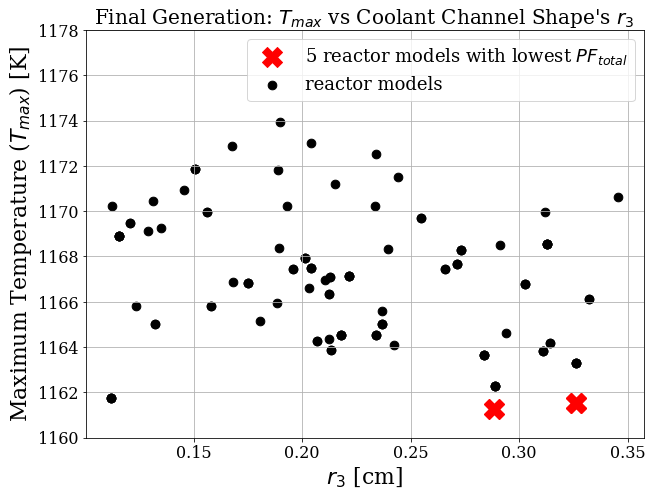
\includegraphics[width=\linewidth]{a-1e-r3.png}
        \caption{Plot of $PF_{total}$ against $r_3$.}
        \label{fig:a-1e-r3} 
    \end{subfigure}
    \begin{subfigure}{0.49\textwidth}
        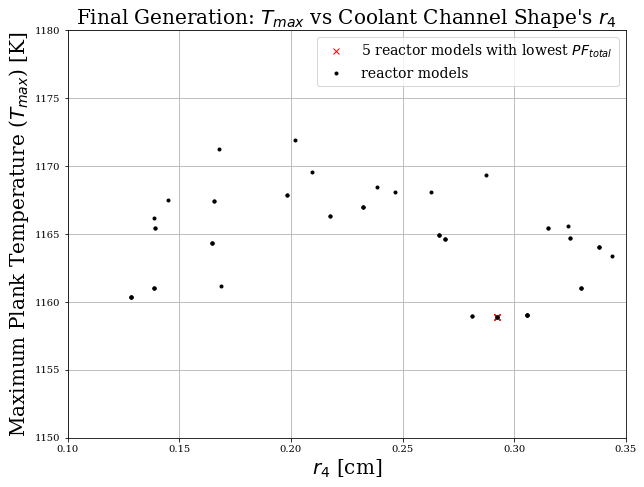
\includegraphics[width=\linewidth]{a-1e-r4.png}
        \caption{Plot of $PF_{total}$ against $r_4$.}
        \label{fig:a-1e-r4} 
    \end{subfigure}
    \begin{subfigure}{0.49\textwidth}
        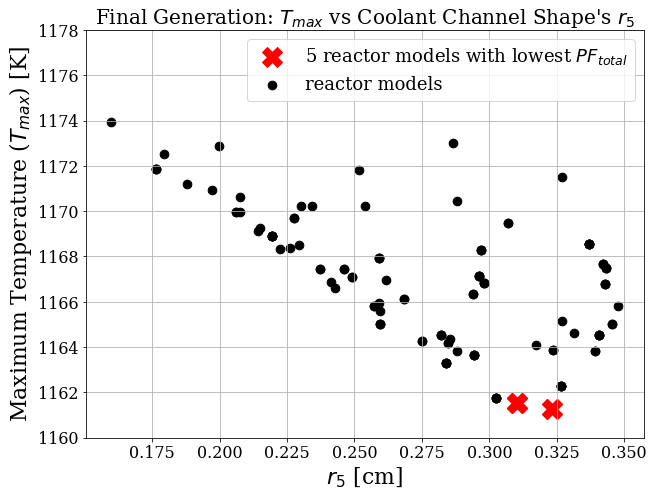
\includegraphics[width=\linewidth]{a-1e-r5.png}
        \caption{Plot of $PF_{total}$ against $r_5$.}
        \label{fig:a-1e-r5} 
    \end{subfigure}
    \caption{Simulation a-1e -- ROLLO single-objective optimization to minimize 
    maximum one-third assembly temperature ($T_{max}$). 
    Plots of final generation's reactor models $T_{max}$ against 
    coolant channel shape input parameters. 
    Red crosses indicate the five reactor models with the lowest $T_{max}$.
    Input parameters varied: coolant channel shape ($r_1, r_2, r_3, r_4, r_5$).}
\end{figure}

Figures \ref{fig:a-1e-r1} and \ref{fig:a-1e-r5} demonstrate negative linear correlations 
between the one-third assembly's $T_{max}$ with $r_1$ and $r_5$. 
Figures \ref{fig:a-1e-r2}, \ref{fig:a-1e-r3} and \ref{fig:a-1e-r4} demonstrate that 
there is no correlation between $T_{max}$ with $r_2$, $r_3$, and $r_4$. 
% TODO rerun with higher PF and larger generations 

\subsection{Objective: Minimize Fuel-Normalized Power Peaking Factor ($PPF_{fuel}$)}
\label{sec:assem-1-obj-ppf}
This section reports the minimize fuel-normalized power peaking factor 
($PPF_{fuel}$) single-objective optimization simulation results: a-1c and a-1f. 
Simulation a-1c varies \gls{TRISO} packing fraction distribution 
($\rho_{TRISO}(\vec{r})$), while simulation a-1f varies the coolant channel shape.

\subsubsection{Simulation a-1c: Variation of $\rho_{TRISO}(\vec{r})$}
Table \ref{tab:simulationa1c} shows simulation a-1c's optimization problem parameters. 
\begin{table}[htbp!]
    \centering
    \onehalfspacing
    \caption{Simulation a-1c Optimization Problem Parameters}
	\label{tab:simulationa1c}
    \footnotesize
    \begin{tabular}{l|p{5.3cm}}
    \hline 
    \multicolumn{2}{c}{\textbf{Single Objective: Simulation a-1c}} \\
    \hline 
    \textbf{Objectives} & Minimize $PPF_{fuel}$ \\
    \hline 
    \textbf{Input Parameter variations}
    & $\rho_{TRISO}(\vec{r})$: $0<a<2$, $0<d<2$\\
    & $\rho_{TRISO}(\vec{r})$: $0<b<\frac{\pi}{2}$, $0<e<\frac{\pi}{2}$\\
    & $\rho_{TRISO}(\vec{r})$: $0<c<2\pi$, $0<f<2\pi$\\
    \hline
    \textbf{Constraints} & $k_{eff} \geq 1.38$\\ 
    & $PF_{total}$ = 0.06 \\
    \hline 
    \textbf{Genetic Algorithm Parameters} & Population size: 128 \\
    & Generations: 2 \\
    \hline
    \end{tabular}
\end{table}

Figure \ref{fig:assem-obj-1-ppf-evol} shows the one-third assembly's $PPF_{fuel}$ 
evolution. 
Figure \ref{fig:assem-obj-1-ppf-final} shows the four unique TRISO packing fraction 
distributions in the final generation with the most minimized $PPF_{fuel}$. 
Figure \ref{fig:assem-obj-1-ppf-most-minimized} illustrates the \gls{AHTR} one-third 
assembly model with the most-minimized $PPF_{fuel}$. 
\begin{figure}[htbp!]
    \centering
    \begin{subfigure}{\textwidth}
        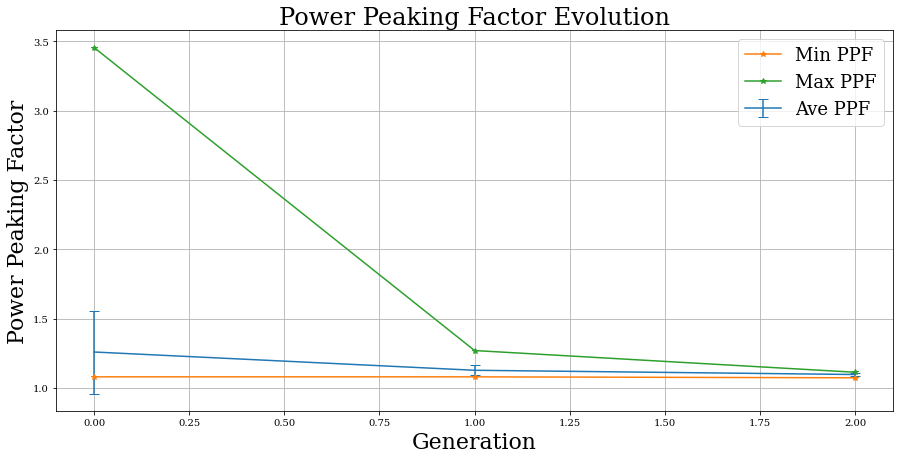
\includegraphics[width=\linewidth]{assem-obj-1-ppf-evol.png}
        \caption{Minimum, average, and maximum evolution of $PPF_{fuel}$ in the 
        AHTR one-third assembly.}
        \label{fig:assem-obj-1-ppf-evol} 
    \end{subfigure}
    \begin{subfigure}{\textwidth}
        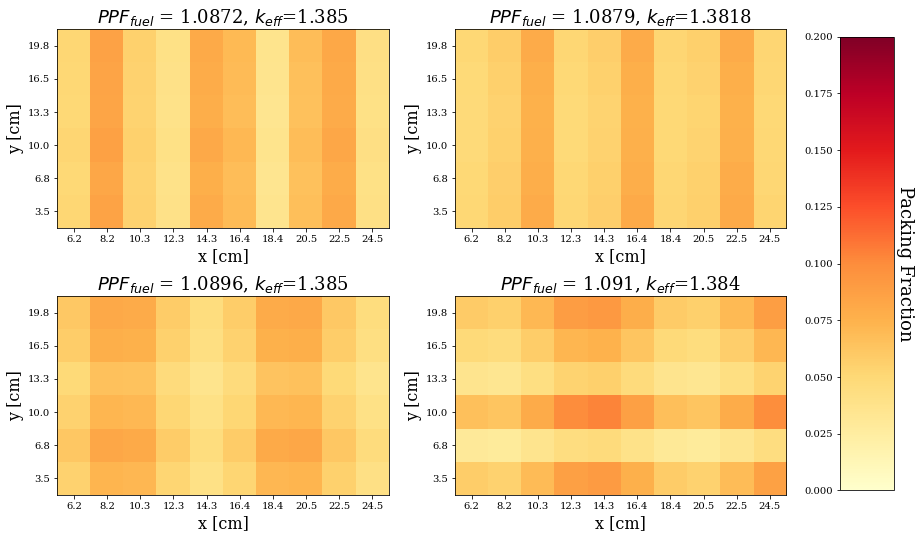
\includegraphics[width=\linewidth]{assem-obj-1-ppf-final.png}
        \caption{TRISO distribution for the four unique reactor models with the 
        lowest $PPF_{fuel}$ in the AHTR one-third assembly at the final generation.}
        \label{fig:assem-obj-1-ppf-final} 
    \end{subfigure}
    \caption{Simulation a-1c -- ROLLO single-objective optimization to minimize 
    AHTR one-third assembly's fuel-normalized power peaking factor ($PPF_{fuel}$). 
    Input parameters varied: TRISO distribution ($\rho_{TRISO}(\vec{r})$).
    $PF_{total}$ = 0.06.}
    \label{fig:assem-obj-1-ppf}
\end{figure}
\begin{figure}[htbp!]
    \ContinuedFloat
    \centering
    \begin{subfigure}{\textwidth}
        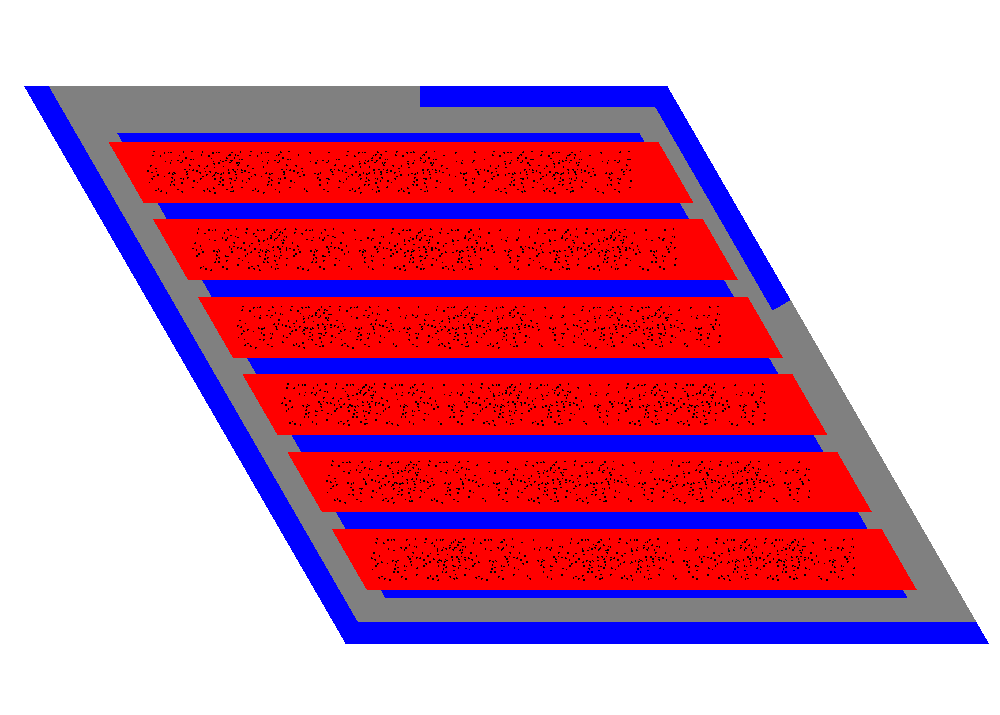
\includegraphics[width=0.7\linewidth]{assem-obj-1-ppf-most-minimized.png}
        \caption{\gls{AHTR} one-third assembly model with the most-minimized 
        $PPF_{fuel}$, corresponding to the the first TRISO distribution in Figure 
        \ref{fig:assem-obj-1-ppf-final}. The reactor model has $PPF_{fuel}=1.0872$
        and $k_{eff}=1.385$.}
        \label{fig:assem-obj-1-ppf-most-minimized} 
    \end{subfigure}
    \caption{Simulation a-1c -- ROLLO single-objective optimization to minimize 
    AHTR one-third assembly's fuel-normalized power peaking factor ($PPF_{fuel}$). 
    Input parameters varied: TRISO distribution ($\rho_{TRISO}(\vec{r})$).
    $PF_{total}$ = 0.06.}
\end{figure}

Figure \ref{fig:assem-obj-1-ppf-evol} shows that the minimum and average 
one-third assembly's $T_{max}$ converged to approximately 1.1.
In Figure \ref{fig:assem-obj-1-ppf-final}, the most-minimized TRISO distribution has 
a $PPF_{fuel} = 1.0872$ and an oscillating TRISO distribution along the x-axis and a 
packing fraction standard deviation of $0.017$ across the one-third assembly. 
Along the x-axis, the distribution peaks at the 2nd, 5th, and 9th fuel 
cell columns (at 8.2cm, 14.3cm, and 22.5cm) with $PF\approx0.08$ and has minimum points
at the 4th and 7th fuel cell columns (at 12.3cm and 18.4cm) with $PF\approx0.035$. 

\subsubsection{Simulation a-1f: Variation of Coolant channel shape}
Table \ref{tab:simulationa1f} shows simulation a-1f's optimization problem parameters. 
\begin{table}[htbp!]
    \centering
    \onehalfspacing
    \caption{Simulation a-1f Optimization Problem Parameters}
	\label{tab:simulationa1f}
    \footnotesize
    \begin{tabular}{l|p{6cm}}
    \hline 
    \multicolumn{2}{c}{\textbf{Single Objective: Simulation a-1f}} \\
    \hline 
    \textbf{Objectives} & Minimize $PPF_{fuel}$ \\
    \hline 
    \textbf{Input Parameter variations} 
    & coolant channel shape: $0.05<r_{1}<0.35$ \\
    & coolant channel shape: $0.05<r_{2}<0.35$ \\
    & coolant channel shape: $0.05<r_{3}<0.35$ \\
    & coolant channel shape: $0.05<r_{4}<0.35$ \\
    & coolant channel shape: $0.05<r_{5}<0.35$ \\
    \hline
    \textbf{Constraints} & $k_{eff} \geq 1.38$\\ 
    & $PF_{total}$ = 0.04 \\
    \hline 
    \textbf{Genetic Algorithm Parameters} & Population size: 64 \\
    & Generations: 2 \\
    \hline
    \end{tabular}
\end{table}

Figure \ref{fig:a-1f} shows the plots of coolant channel shape's 
$r_1, r_2, r_3, r_4,$ and $r_5$ values against $PPF_{fuel}$. 
\begin{figure}[htbp!]
    \centering
    \begin{subfigure}{0.49\textwidth}
        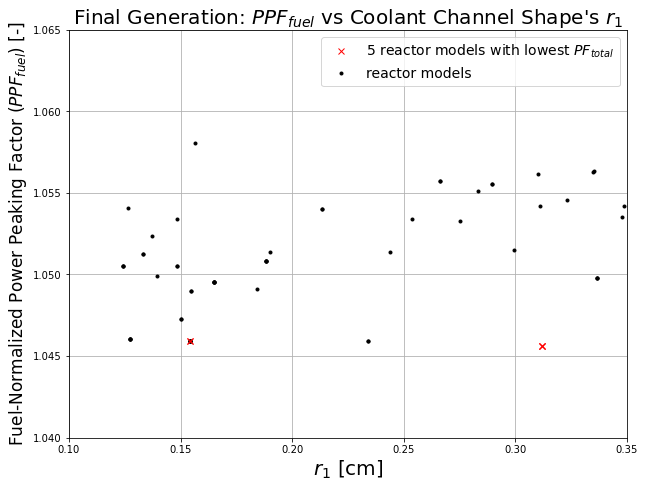
\includegraphics[width=\linewidth]{a-1f-r1.png}
        \caption{Plot of $PF_{total}$ against $r_1$.}
        \label{fig:a-1f-r1} 
    \end{subfigure}
    \begin{subfigure}{0.49\textwidth}
        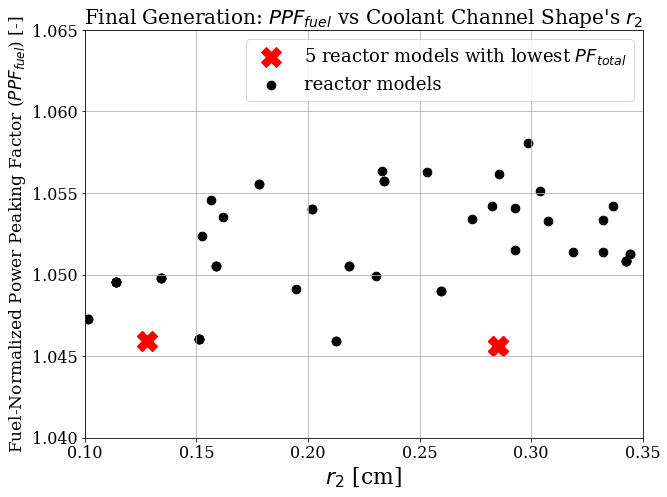
\includegraphics[width=\linewidth]{a-1f-r2.png}
        \caption{Plot of $PF_{total}$ against $r_2$.}
        \label{fig:a-1f-r2} 
    \end{subfigure}
    \begin{subfigure}{0.49\textwidth}
        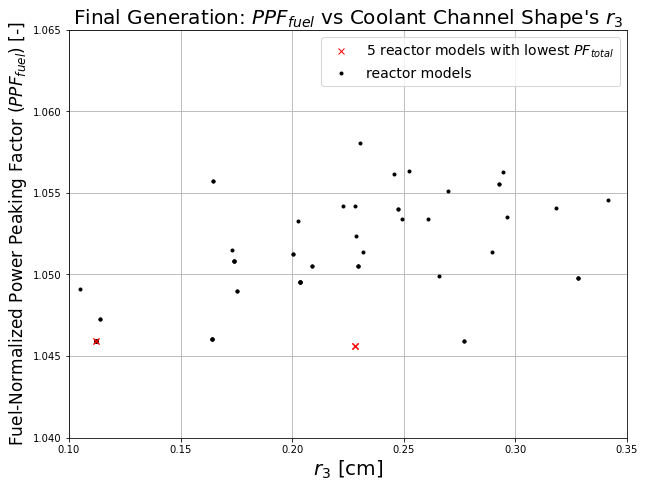
\includegraphics[width=\linewidth]{a-1f-r3.png}
        \caption{Plot of $PF_{total}$ against $r_3$.}
        \label{fig:a-1f-r3} 
    \end{subfigure}
    \begin{subfigure}{0.49\textwidth}
        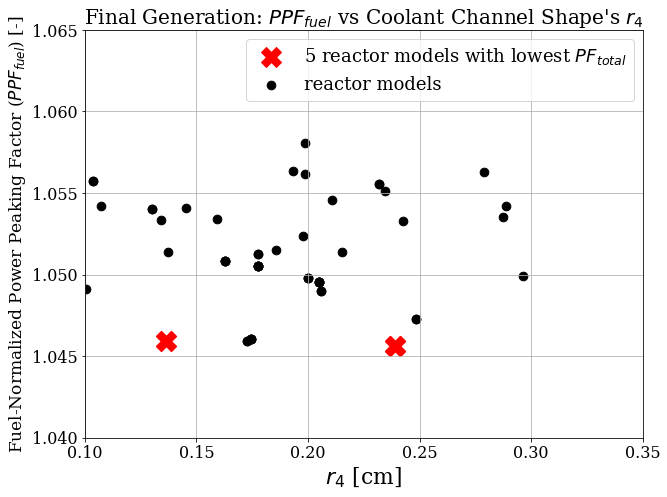
\includegraphics[width=\linewidth]{a-1f-r4.png}
        \caption{Plot of $PF_{total}$ against $r_4$.}
        \label{fig:a-1f-r4} 
    \end{subfigure}
    \begin{subfigure}{0.49\textwidth}
        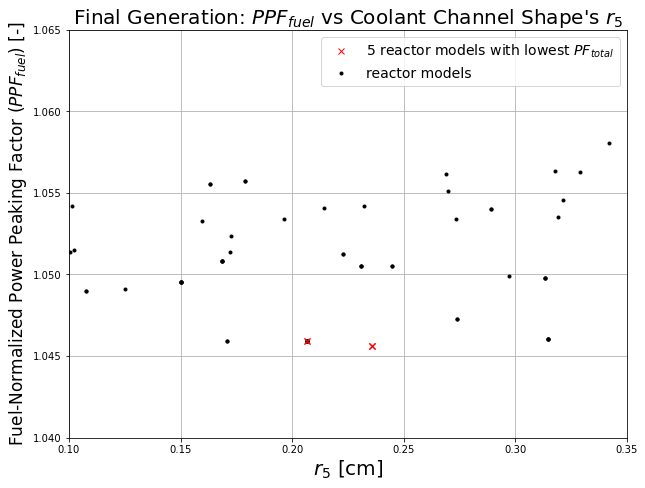
\includegraphics[width=\linewidth]{a-1f-r5.png}
        \caption{Plot of $PF_{total}$ against $r_5$.}
        \label{fig:a-1f-r5} 
    \end{subfigure}
    \caption{Simulation a-1f -- ROLLO single-objective optimization to minimize 
    AHTR one-third assembly's fuel-normalized power peaking factor ($PPF_{fuel}$). 
    Plots of simulation a-1f final generation's reactor models $PPF_{fuel}$ against 
    coolant channel shape input parameters. 
    Red crosses indicate the five reactor models with the lowest $PPF_{fuel}$.
    Input parameters varied: total fuel packing fraction 
    ($PPF_{fuel}$), and coolant channel shape ($r_1, r_2, r_3, r_4, r_5$).}
    \label{fig:a-1f}
\end{figure}

Figure \ref{fig:a-1f} demonstrates that there is no correlation between $PPF_{fuel}$ 
and coolant channel shape's $r_1, r_2, r_3, r_4,$ and $r_5$. 

\pagebreak
\section{AHTR One-Third Assembly: Two-Objective Optimization Results}
In this section, I report the \gls{AHTR} one-third assembly's \gls{ROLLO} two-objective 
optimization results. 
The previous section's one-objective optimization results inform the multi-objective 
optimization simulations in this section and Section \ref{assem-three-obj}.
Table \ref{tab:assem-obj-breakdown} summarized the two-objective simulations in this 
section: a-2a, a-2b, and a-2c.

\subsection{a-2a: Minimize $PF_{total}$ and $T_{max}$}
\label{sec:a-2a}
This section reports results from the two-objective optimization simulation a-2a, the 
objectives minimized are total fuel packing fraction ($PF_{total}$) and maximum one-third 
assembly temperature ($T_{max}$).  
Table \ref{tab:simulationa2a} shows simulation a-2a's optimization problem parameters. 
\begin{table}[htbp!]
    \centering
    \onehalfspacing
    \caption{Simulation a-2a Optimization Problem Parameters}
	\label{tab:simulationa2a}
    \footnotesize
    \begin{tabular}{l|p{5.3cm}}
    \hline 
    \multicolumn{2}{c}{\textbf{Two Objectives: Simulation a-2a}} \\
    \hline 
    \textbf{Objectives} & Minimize $PF_{total}$ \\
    & Minimize $T_{max}$ \\
    \hline 
    \textbf{Input parameter variations} & $0.05<PF_{total}<0.07$ \\
    & $\rho_{TRISO}(\vec{r})$: $0<a<2$, $0<d<2$\\
    & $\rho_{TRISO}(\vec{r})$: $0<b<\frac{\pi}{2}$, $0<e<\frac{\pi}{2}$\\
    & $\rho_{TRISO}(\vec{r})$: $0<c<2\pi$, $0<f<2\pi$\\
    \hline
    \textbf{Constraints} & $k_{eff} \geq 1.38$\\ 
    \hline 
    \textbf{Genetic algorithm parameters} & Population size: 128 \\
    & Generations: 3 \\
    \hline
    \end{tabular}
\end{table}

Table \ref{tab:a2a-hypervolume} shows the hypervolume value at each generation, 
confirming that simulation a-2a converges by generation 3. 
\begin{table}[htbp!]
    \centering
    \onehalfspacing
    \caption{Simulation a-2a hypervolume values at each generation.}
	\label{tab:a2a-hypervolume}
    \footnotesize
    \begin{tabular}{ll}
    \hline 
    \multicolumn{2}{c}{\textbf{Two Objectives: Simulation a-2a}} \\
    \multicolumn{2}{c}{Reference point: (0.07, 1700)} \\
    \hline 
    \textbf{Generation} & \textbf{Hypervolume [-]} \\
    \hline
    1 & 6.0090 \\
    2 & 6.0859 \\
    3 & 6.2220 \\
    \hline
    \end{tabular}
\end{table}

Figure \ref{fig:assem-obj-2-pftemp-pareto} shows a plot of the final generation's reactor 
models' $PF_{total}$ against $T_{max}$, crosses mark the reactor models that fall on 
the Pareto front.
Figure \ref{fig:assem-obj-2-pftemp-pareto-distr} shows the 13 TRISO packing fraction 
distributions in the final generation that fall on the Pareto front. 
\begin{figure}[htbp!]
    \begin{subfigure}{\textwidth}
        \centering
        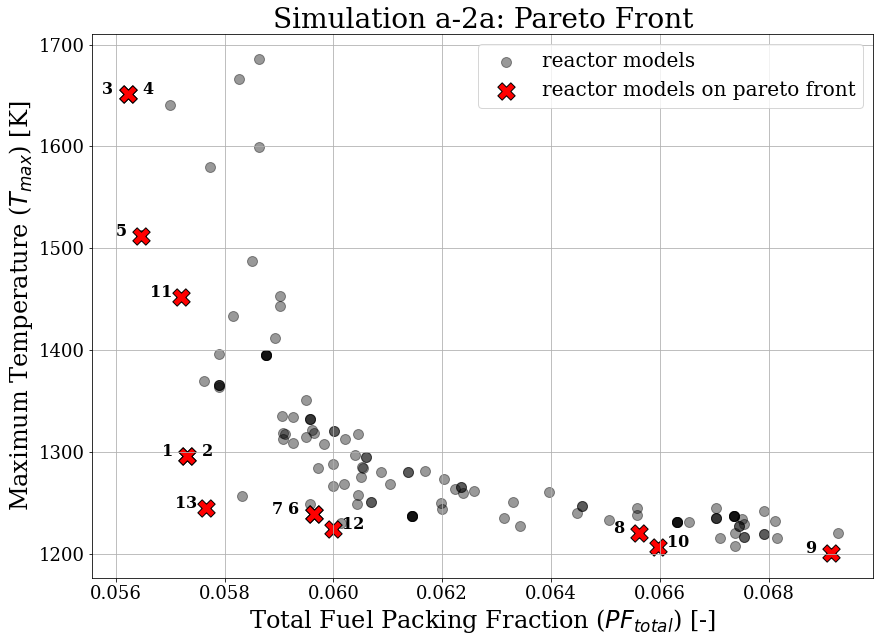
\includegraphics[width=0.9\linewidth]{assem-obj-2-pftemp-pareto.png}
        \caption{Plot of final generation's reactor models' $PF_{total}$ against 
        $T_{max}$. 
        Crosses indicate the reactor models on the Pareto front. Annotated numbers 
        on each cross correspond to TRISO distributions in the plot below.}
        \label{fig:assem-obj-2-pftemp-pareto} 
    \end{subfigure}
    \begin{subfigure}{\textwidth}
        \centering
        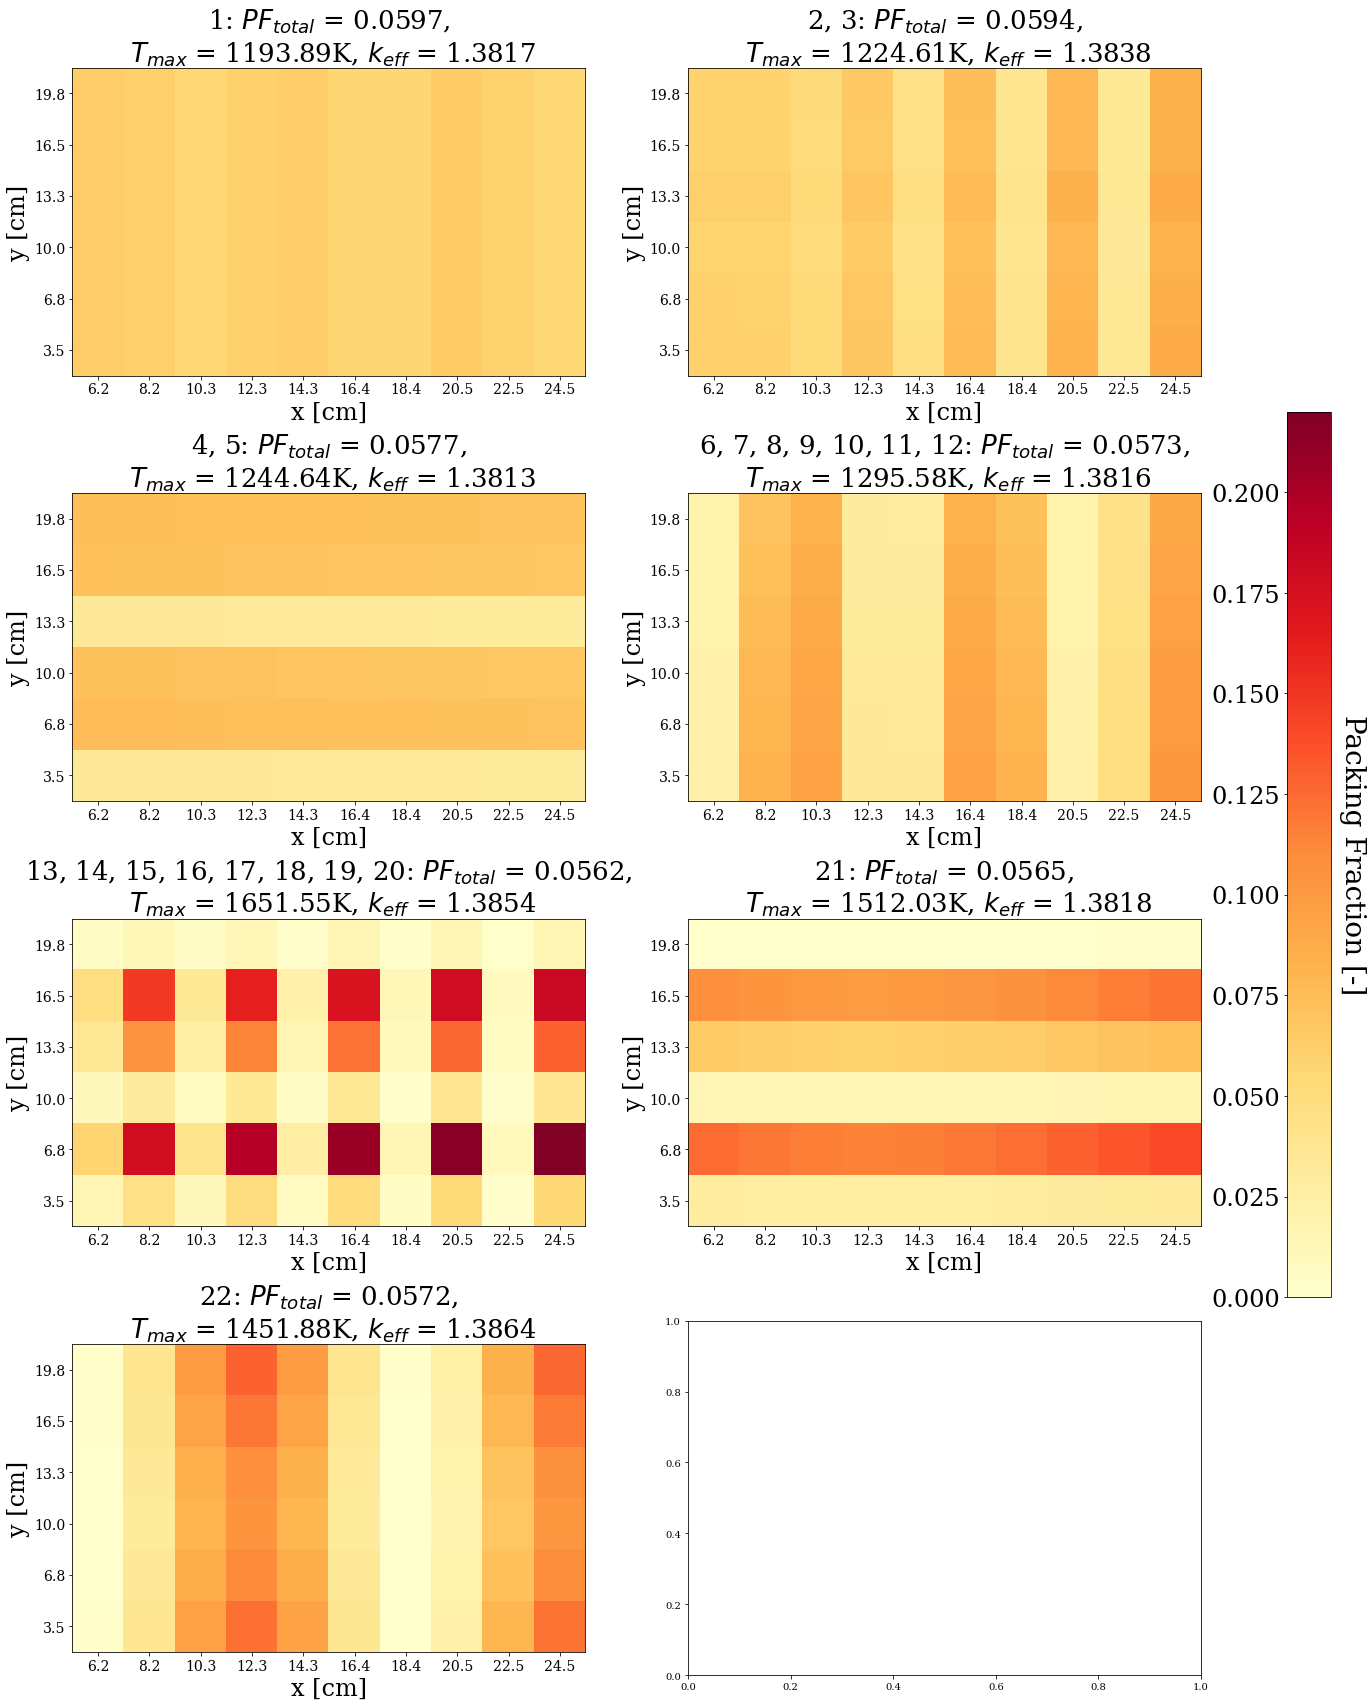
\includegraphics[width=\linewidth]{assem-obj-2-pftemp-pareto-distr.png}
        \caption{TRISO distribution for the 13 reactor models on the Pareto front.
        Numbered reactor models correspond to numbered crosses in the plot above. }
        \label{fig:assem-obj-2-pftemp-pareto-distr} 
    \end{subfigure}
    \caption{Simulation a-2a -- ROLLO two-objective optimization to minimize total fuel 
    packing fraction ($PF_{total}$) and one-third assembly's maximum temperature ($T_{max}$). 
    Input parameters varied: total fuel packing fraction ($PF_{total}$) and TRISO 
    packing fraction distribution ($\rho_{TRISO}(\vec{r})$).}
    \label{fig:assem-obj-2-pftemp}
\end{figure}

Figure \ref{fig:assem-obj-2-pftemp-pareto} shows that minimize $PF_{total}$ and 
minimize $T_{max}$ are contrasting objectives. 

In Figure \ref{fig:assem-obj-2-pftemp}, the one-third assembly model with the 
most-minimized $PF_{total}$ and highest $T_{max}$ is reactor models 3 and 4. 
Both models have an oscillating TRISO distribution along the both the 
x-axis and y-axis, and a packing fraction standard deviation of $0.066$ across the 
one-third assembly. 
Along the x-axis, the distribution peaks at the even fuel cell columns (at 8.2cm,  
and 12.3cm, 14.3cm, 16.4cm, 18.4cm, 20.5cm, 22.5cm, and 24.5cm) and has 
minimum points at the odd fuel cell columns (at 6.2cm, 10.3cm, 14.3cm, 18.4cm,
and 22.5cm).
The even fuel cell columns have a $\sim0.18$ y-axis variation. 

In Figure \ref{fig:assem-obj-2-pftemp}, the one-third assembly model with the 
most-minimized $T_{max}$ and highest $PF_{total}$ is reactor model 9. 
Reactor model 9 has an almost constant TRISO packing fraction distribution. 
% maybe do a zoom in with a different scale. to compare to a-1b. 

The one-third assembly model that visually from the Pareto Front (Figure 
\ref{fig:assem-obj-2-pftemp-pareto}) minimizes both $PF_{total}$ and $T_{max}$ 
to an equal extent is reactor model 13. 
Reactor model 13 has an oscillating TRISO distribution along the y-axis and 
a packing fraction standard deviation of $0.066$ across the one-third assembly. 
Along the y-axis, the distribution peaks at the 2nd, 3rd, 5th, and 6th rows 
(at 6.8cm, 10.0cm, 16.5cm, and 19.8cm) with $PF\approx0.07$ and has minimum points at 
the 1st and 4th rows (at 3.5cm and 13.3cm) with $PF\approx0.03$. 

\subsection{a-2b: Minimize $PF_{total}$ and $PPF_{fuel}$}
\label{sec:a-2b}
This section reports results from the two-objective optimization simulation a-2b, the 
objectives minimized are total fuel packing fraction ($PF_{total}$) and fuel-normalized 
power peaking factor ($PPF_{fuel}$).  
Table \ref{tab:simulationa2b} shows simulation a-2b's optimization problem parameters. 
\begin{table}[htbp!]
    \centering
    \onehalfspacing
    \caption{Simulation a-2b Optimization Problem Parameters}
	\label{tab:simulationa2b}
    \footnotesize
    \begin{tabular}{l|p{5.3cm}}
    \hline 
    \multicolumn{2}{c}{\textbf{Two Objectives: Simulation a-2b}} \\
    \hline 
    \textbf{Objectives} & Minimize $PF_{total}$ \\
    & Minimize $PPF_{fuel}$ \\
    \hline 
    \textbf{Input parameter variations} & $0.05<PF_{total}<0.07$ \\
    & $\rho_{TRISO}(\vec{r})$: $0<a<2$, $0<d<2$\\
    & $\rho_{TRISO}(\vec{r})$: $0<b<\frac{\pi}{2}$, $0<e<\frac{\pi}{2}$\\
    & $\rho_{TRISO}(\vec{r})$: $0<c<2\pi$, $0<f<2\pi$\\
    \hline
    \textbf{Constraints} & $k_{eff} \geq 1.38$\\ 
    \hline 
    \textbf{Genetic algorithm parameters} & Population size: 128 \\
    & Generations: 3 \\
    \hline
    \end{tabular}
\end{table}

Table \ref{tab:a2b-hypervolume} shows the hypervolume value at each generation, 
confirming that simulation a-2b converges by generation 3. 
\begin{table}[htbp!]
    \centering
    \onehalfspacing
    \caption{Simulation a-2b hypervolume values at each generation.}
	\label{tab:a2b-hypervolume}
    \footnotesize
    \begin{tabular}{ll}
    \hline 
    \multicolumn{2}{c}{\textbf{Two Objectives: Simulation a-2b}} \\
    \multicolumn{2}{c}{Reference point: (0.07, 1.9)} \\
    \hline 
    \textbf{Generation} & \textbf{Hypervolume [-]} \\
    \hline
    1 & 0.00989 \\
    2 & 0.00991 \\
    3 & 0.00997 \\
    \hline
    \end{tabular}
\end{table}

Figure \ref{fig:assem-obj-2-pfppf-pareto} shows a plot of the final generation's reactor 
models' $PF_{total}$ against $PPF_{fuel}$, crosses mark the reactor models that fall on 
the Pareto front.
Figure \ref{fig:assem-obj-2-pfppf-pareto-distr} shows the 6 TRISO packing fraction 
distributions in the final generation that fall on the Pareto front. 
\begin{figure}[htbp!]
    \begin{subfigure}{\textwidth}
        \centering
        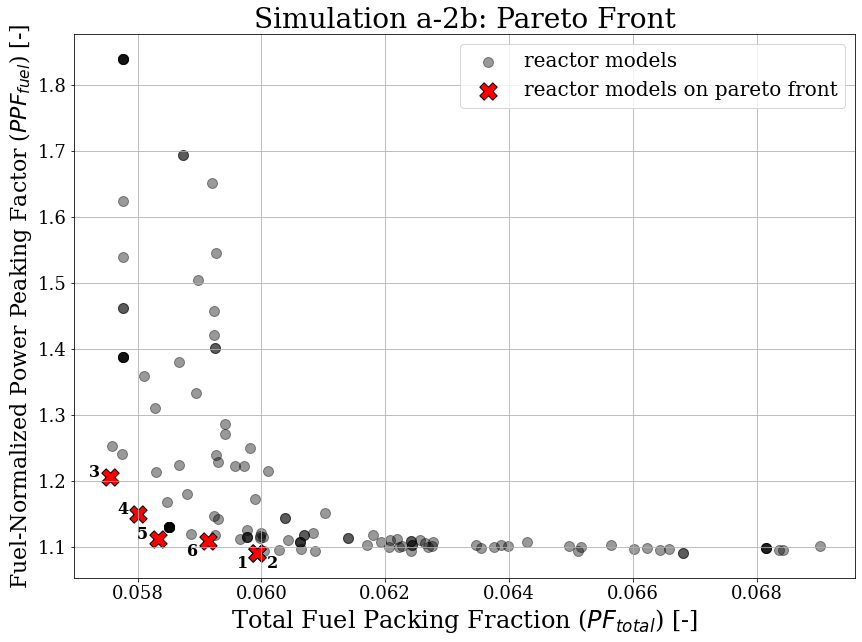
\includegraphics[width=\linewidth]{assem-obj-2-pfppf-pareto.png}
        \caption{Plot of final generation's reactor models' $PF_{total}$ against 
        $PPF_{fuel}$. 
        Crosses indicate the reactor models on the Pareto front. Annotated numbers 
        on each cross correspond to TRISO distributions in the plot below.}
        \label{fig:assem-obj-2-pfppf-pareto} 
    \end{subfigure}
    \begin{subfigure}{\textwidth}
        \centering
        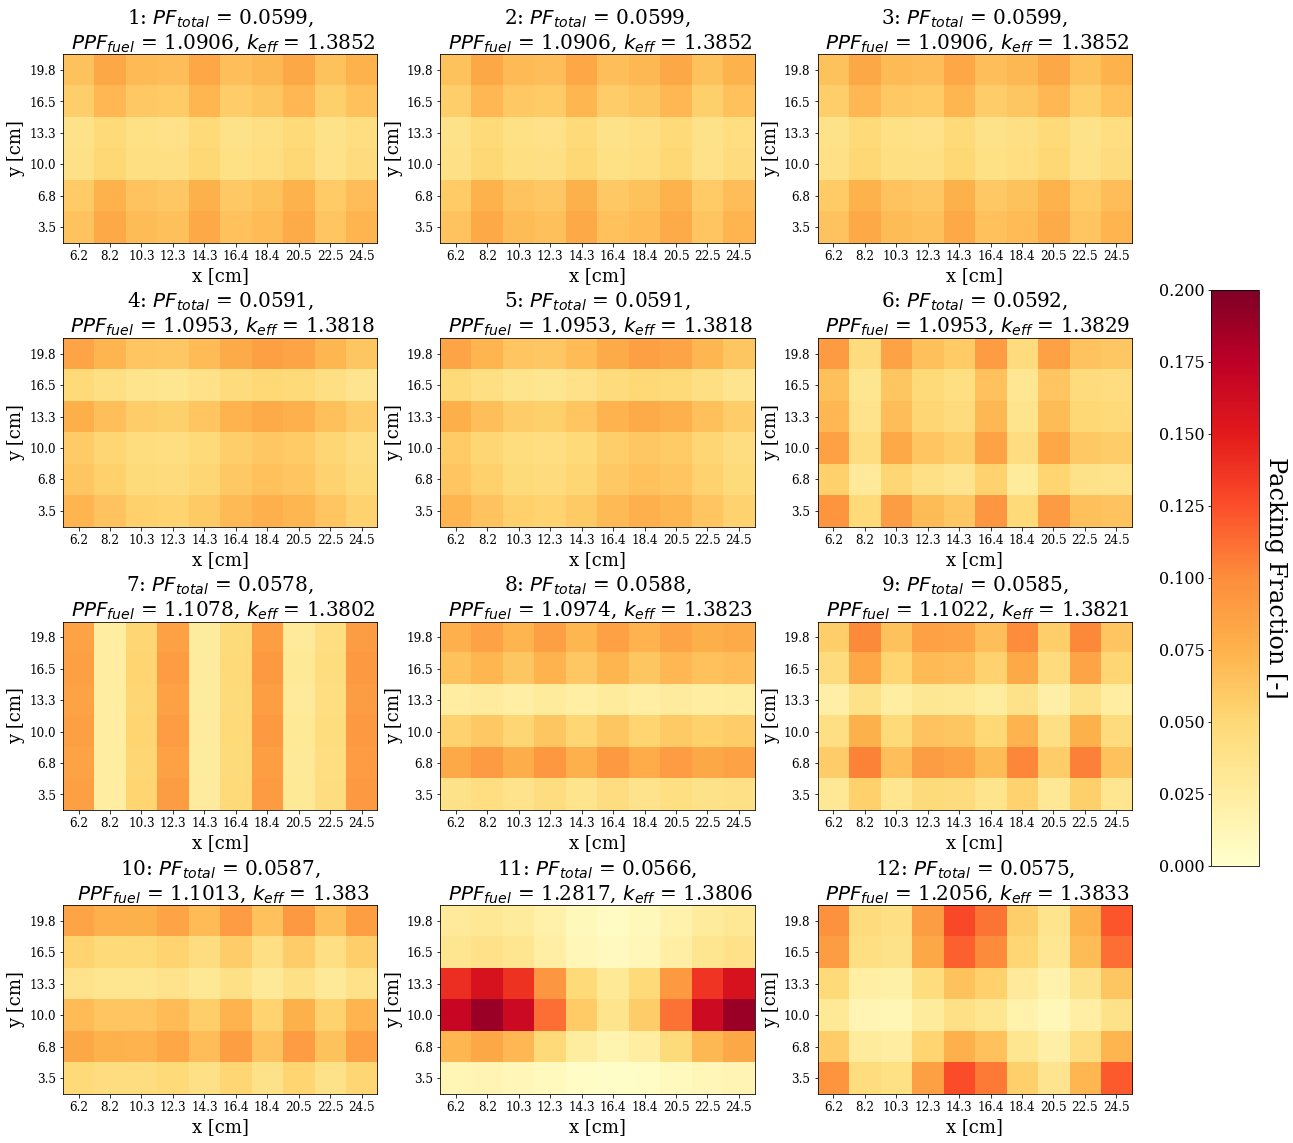
\includegraphics[width=\linewidth]{assem-obj-2-pfppf-pareto-distr.png}
        \caption{TRISO distribution for the 6 reactor models on the Pareto front.
        Numbered reactor models correspond to numbered crosses in the plot above. }
        \label{fig:assem-obj-2-pfppf-pareto-distr} 
    \end{subfigure}
    \caption{Simulation a-2b -- ROLLO two-objective optimization to minimize total fuel 
    packing fraction ($PF_{total}$) and normalized power peaking factor ($PPF_{fuel}$) 
    in the \gls{AHTR} one-third assembly. 
    Input parameters varied: total fuel packing fraction ($PF_{total}$) and TRISO 
    packing fraction distribution ($\rho_{TRISO}(\vec{r})$).}
    \label{fig:assem-obj-2-pfppf}
\end{figure}

Figure \ref{fig:assem-obj-2-pfppf-pareto} shows that minimize $PF_{total}$ and 
minimize $PPF_{fuel}$ are contrasting objectives. 

In Figure \ref{fig:assem-obj-2-pfppf}, the one-third assembly model with 
the most-minimized $PF_{total}$ and highest $PPF_{fuel}$ is reactor model 3. 
Reactor model 3 has an oscillating TRISO distribution along the both the 
x-axis and y-axis, and a packing fraction standard deviation of $0.032$ across the 
one-third assembly. 
Along the x-axis, the distribution peaks at the 5th and 10th fuel cell columns (at 14.3cm 
and 24.5cm) and has minimum points at the 2nd, 3rd, and 8th columns (at 8.2cm, 10.3cm, 
and 20.5cm).
The 5th and 10th columns have the largest y-axis variation of $\sim0.09$ and the 
2nd, 3rd, and 8th columns have the smallest y-axis variation of $\sim0.03$.
Along the y-axis, the distribution peaks at the top and bottom row (at 3.5cm and 
19.8cm) and has a minimum point at the 3rd row (at 10.0cm). 
The top and bottom row have the largest x-axis variation of $\sim0.09$ and the 3rd row 
has the smallest x-axis variation of $\sim0.03$. 

In Figure \ref{fig:assem-obj-2-pfppf}, the one-third assembly model with 
the most-minimized $PPF_{fuel}$ and highest $PF_{total}$ is reactor model 1.
Reactor model 1 has an oscillating TRISO distribution along the both the 
x-axis and y-axis and a packing fraction standard deviation of $0.013$ across the 
one-third assembly.
Along the x-axis, the distribution peaks at the 2nd, 5th, and 8th fuel cell columns (at 
8.2cm, 14.3cm, and 20.5cm) and has minimum points at the 1st, 6th, and 9th (at 6.2cm, 
16.4cm, and 22.5cm).
The 2nd, 5th, and 8th columns have the largest y-axis variation of $\sim0.034$ and the 
1st, 6th, and 9th columns have the smallest y-axis variation of $\sim0.027$.
On the y-axis, the distribution has peaks at the top and bottom row (at 3.5cm and 
19.8cm) and has a minimum point in the center rows (at 10.0cm and 13.3cm).
The top and bottom row have the largest x-axis variation of $\sim0.018$ and the center rows 
have the smallest x-axis variation of $\sim0.011$. 

The one-third assembly model that visually from the Pareto Front (Figure 
\ref{fig:assem-obj-2-pfppf-pareto}) minimizes both $PF_{total}$ and $PPF_{fuel}$ 
to an equal extent is reactor model 5. 
Similar to reactor models 3 and 1, reactor model 5 has an oscillating TRISO distribution 
along the both the x-axis and y-axis and it has a packing fraction standard deviation 
of $0.02$ across the one-third assembly.
Along the x-axis, the distribution peaks at the 1st, 5th, and 8th fuel cell columns 
(at 6.2cm, 14.3cm, and 20.5cm) and has minimum points at the 3rd, 6th, and 10th fuel 
cell columns (at 10.3cm, 16.4cm, 24.5cm). 
The 1st, 5th, and 8th columns have the largest y-axis variation of $\sim0.014$ and the 
3rd, 6th, and 10th columns have the smallest y-axis variation of $\sim0.006$.
Along the y-axis, the distribution peaks at the 2nd and 4th row (at 6.8cm and 13.3cm). 
All the rows along the y-axis have a similar x-axis variation of $\sim0.06$.

\subsection{a-2c: Minimize $T_{max}$ and $PPF_{fuel}$}
\label{sec:a-2c}
This section reports results from the two-objective optimization simulation a-2c, the 
objectives minimized are maximum one-third assembly temperature ($T_{max}$) and 
fuel-normalized power peaking factor ($PPF_{fuel}$).  
Table \ref{tab:simulationa2c} shows simulation a-2c's optimization problem parameters. 
\begin{table}[htbp!]
    \centering
    \onehalfspacing
    \caption{Simulation a-2c Optimization Problem Parameters}
	\label{tab:simulationa2c}
    \footnotesize
    \begin{tabular}{l|p{5.3cm}}
    \hline 
    \multicolumn{2}{c}{\textbf{Two Objectives: Simulation a-2c}} \\
    \hline 
    \textbf{Objectives} & Minimize $T_{max}$ \\
    & Minimize $PPF_{fuel}$ \\
    \hline 
    \textbf{Input parameter variations}
    & $\rho_{TRISO}(\vec{r})$: $0<a<2$, $0<d<2$\\
    & $\rho_{TRISO}(\vec{r})$: $0<b<\frac{\pi}{2}$, $0<e<\frac{\pi}{2}$\\
    & $\rho_{TRISO}(\vec{r})$: $0<c<2\pi$, $0<f<2\pi$\\
    \hline
    \textbf{Constraints} & $k_{eff} \geq 1.38$\\ 
    & $PF_{total} = 0.06$\\
    \hline 
    \textbf{Genetic algorithm parameters} & Population size: 128 \\
    & Generations: 2 \\
    \hline
    \end{tabular}
\end{table}

Table \ref{tab:a2c-hypervolume} shows the hypervolume value at each generation, 
confirming that simulation a-2c converges by generation 2. 
\begin{table}[htbp!]
    \centering
    \onehalfspacing
    \caption{Simulation a-2c hypervolume values at each generation.}
	\label{tab:a2c-hypervolume}
    \footnotesize
    \begin{tabular}{ll}
    \hline 
    \multicolumn{2}{c}{\textbf{Two Objectives: Simulation a-2c}} \\
    \multicolumn{2}{c}{Reference point: (1700, 1.5)} \\
    \hline 
    \textbf{Generation} & \textbf{Hypervolume [-]} \\
    \hline
    1 & 210.685 \\
    2 & 210.685 \\
    \hline
    \end{tabular}
\end{table}

Figure \ref{fig:assem-obj-2-tempppf-pareto} shows a plot of the final generation's reactor 
models' $T_{max}$ against $PPF_{fuel}$, crosses mark the reactor models that fall on 
the Pareto front.
Figure \ref{fig:assem-obj-2-tempppf-pareto-distr} shows the 1 TRISO packing fraction 
distributions in the final generation that fall on the Pareto front. 
\begin{figure}[htbp!]
    \centering
    \begin{subfigure}{\textwidth}
        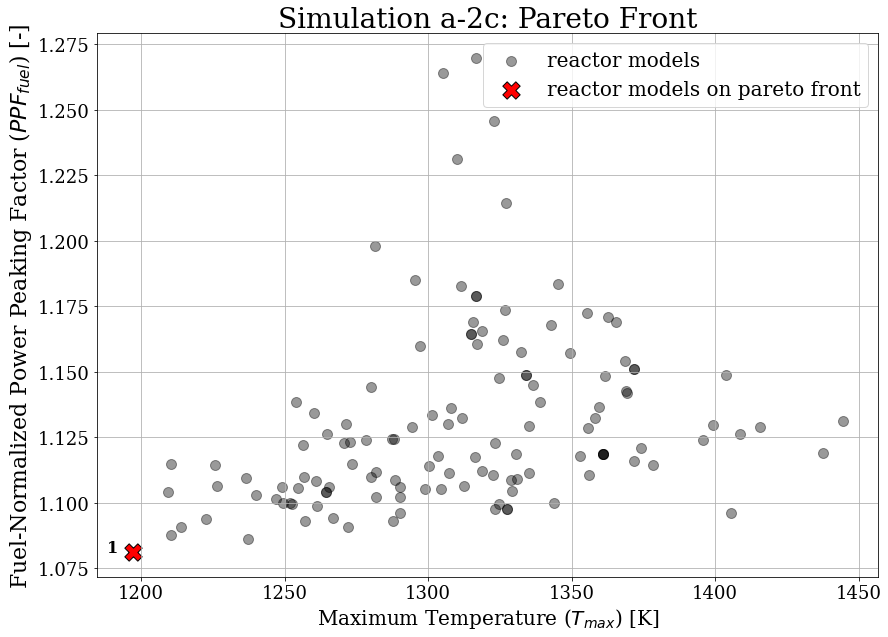
\includegraphics[width=\linewidth]{assem-obj-2-tempppf-pareto.png}
        \caption{Plot of final generation's reactor models' $T_{max}$ against 
        $PPF_{fuel}$. 
        Crosses indicate the reactor models on the Pareto front. Annotated numbers 
        on each cross correspond to TRISO distributions in the plot below.}
        \label{fig:assem-obj-2-tempppf-pareto} 
    \end{subfigure}
    \begin{subfigure}{\textwidth}
        \centering
        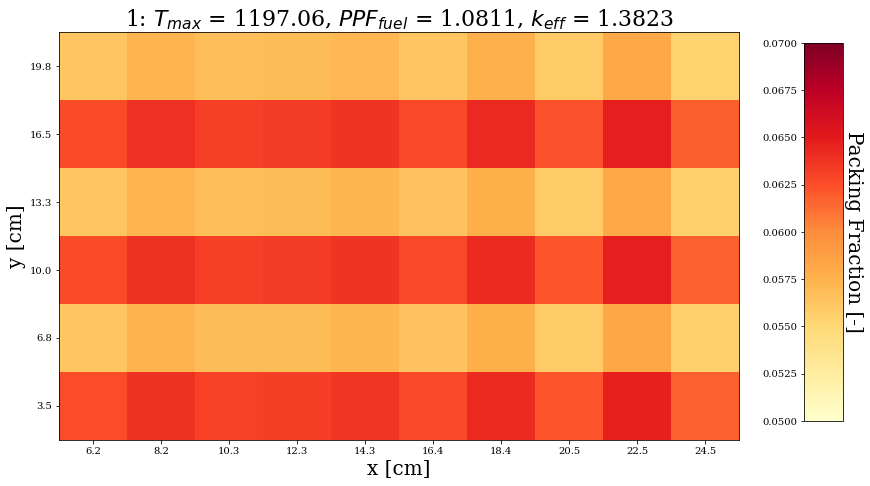
\includegraphics[width=0.8\linewidth]{assem-obj-2-tempppf-pareto-distr.png}
        \caption{TRISO distribution for the 1 reactor models on the Pareto front.
        Numbered reactor models correspond to numbered crosses in the plot above. }
        \label{fig:assem-obj-2-tempppf-pareto-distr} 
    \end{subfigure}
    \caption{Simulation a-2c -- ROLLO two-objective optimization to minimize 
    one-third assembly's maximum temperature ($T_{max}$) and fuel-normalized power peaking factor 
    ($PPF_{fuel}$) in the \gls{AHTR} one-third assembly. 
    Input parameters varied: TRISO packing fraction distribution ($\rho_{TRISO}(\vec{r})$).}
    \label{fig:assem-obj-2-tempppf}
\end{figure}

Figure \ref{fig:assem-obj-2-tempppf-pareto} shows that minimize $T_{max}$ and minimize 
$PPF_{fuel}$ are non-contrasting objectives, resulting in a single reactor model on the 
Pareto Front. 
The TRISO distribution shown in Figure \ref{fig:assem-obj-2-tempppf-pareto-distr} best 
minimizes both $T_{max}$ and $PPF_{fuel}$. 
The reactor model has a TRISO distribution oscillates along the y-axis and oscillates 
slightly on the x-axis, and a packing fraction standard deviation of $0.033$ across 
the one-third assembly. 
The x-axis variation ... 
Along the y-axis, the distribution peaks at the odd rows (at 3.5cm, 10.0cm, and 16.5cm) 
with $PF\approx0.06$ and has minimum points at the even rows (at 6.8cm, 13.3cm, and 19.8cm)
with $PF\approx0.055$.

\pagebreak
\section{AHTR One-Third Assembly: Three-Objective Optimization Results}
\label{assem-three-obj}
This section reports the \gls{AHTR} one-third assembly's \gls{ROLLO} three-objective 
optimization results. 
Table \ref{tab:assem-obj-breakdown} summarized the three-objective simulations in this 
section: a-3a, and a-3b. 

\subsection{a-3a: Variation of $PF_{total}$ and $\rho_{TRISO}(\vec{r})$}
\label{sec:a-3a}
This section reports results from the three-objective optimization simulation a-3a, 
with all objectives minimized: total fuel packing fraction ($PF_{total}$), 
maximum one-third assembly temperature ($T_{max}$), and fuel-normalized power peaking 
factor ($PPF_{fuel}$).  
The input parameters varied are total fuel packing fraction ($PF_{total}$) and 
TRISO packing fraction distribution ($\rho_{TRISO}(\vec{r})$). 
Table \ref{tab:simulationa3a} shows simulation a-3a's optimization problem parameters. 
\begin{table}[htbp!]
    \centering
    \onehalfspacing
    \caption{Simulation a-3a optimization problem parameters.}
	\label{tab:simulationa3a}
    \footnotesize
    \begin{tabular}{l|p{5.3cm}}
    \hline 
    \multicolumn{2}{c}{\textbf{Three Objectives: Simulation a-3a}} \\
    \hline 
    \textbf{Objectives} & Minimize $PF_{total}$ \\
    & Minimize $T_{max}$ \\
    & Minimize $PPF_{fuel}$ \\
    \hline 
    \textbf{Input parameter variations} & $0.05<PF_{total}<0.07$ \\
    & $\rho_{TRISO}(\vec{r})$: $0<a<2$, $0<d<2$\\
    & $\rho_{TRISO}(\vec{r})$: $0<b<\frac{\pi}{2}$, $0<e<\frac{\pi}{2}$\\
    & $\rho_{TRISO}(\vec{r})$: $0<c<2\pi$, $0<f<2\pi$\\
    \hline
    \textbf{Constraints} & $k_{eff} \geq 1.38$\\ 
    \hline 
    \textbf{Genetic algorithm parameters} & Population size: 128 \\
    & Generations: xx \\
    \hline
    \end{tabular}
\end{table}

Table \ref{tab:a3a-hypervolume} shows the hypervolume value at each generation, 
confirming that simulation a-3a converges by generation xx. 
\begin{table}[htbp!]
    \centering
    \onehalfspacing
    \caption{Simulation a-3a hypervolume values at each generation.}
	\label{tab:a3a-hypervolume}
    \footnotesize
    \begin{tabular}{ll}
    \hline 
    \multicolumn{2}{c}{\textbf{Three Objectives: Simulation a-3a}} \\
    \multicolumn{2}{c}{Reference point: (0.06, 1260 ,1.5)} \\
    \hline 
    \textbf{Generation} & \textbf{Hypervolume [-]} \\
    \hline
    1 & xx \\
    2 & xx \\
    3 & xx \\
    4 & xx \\
    5 & xx \\
    \hline
    \end{tabular}
\end{table}

\subsection{a-3b: Variation of $PF_{total}$, $\rho_{TRISO}(\vec{r})$, and Coolant 
Channel Shape}
\label{sec:a-3b}
This section reports results from the three-objective optimization simulation a-3b, 
with all objectives minimized: total fuel packing fraction ($PF_{total}$), maximum 
one-third assembly temperature ($T_{max}$), and fuel-normalized power peaking factor 
($PPF_{fuel}$).  
The input parameters varied are total fuel packing fraction ($PF_{total}$), 
TRISO packing fraction distribution ($\rho_{TRISO}(\vec{r})$), and coolant channel 
shape.  
Table \ref{tab:simulationa3b} shows simulation a-3b's optimization problem parameters. 
\begin{table}[htbp!]
    \centering
    \onehalfspacing
    \caption{Simulation a-3b optimization problem parameters.}
	\label{tab:simulationa3b}
    \footnotesize
    \begin{tabular}{l|p{6.5cm}}
    \hline 
    \multicolumn{2}{c}{\textbf{Three Objectives: Simulation a-3b}} \\
    \hline 
    \textbf{Objectives} & Minimize $PF_{total}$ \\
    & Minimize $T_{max}$ \\
    & Minimize $PPF_{fuel}$ \\
    \hline 
    \textbf{Input parameter variations} & $0.05<PF_{total}<0.07$ \\
    & $\rho_{TRISO}(\vec{r})$: $0<a<2$, $0<d<2$\\
    & $\rho_{TRISO}(\vec{r})$: $0<b<\frac{\pi}{2}$, $0<e<\frac{\pi}{2}$\\
    & $\rho_{TRISO}(\vec{r})$: $0<c<2\pi$, $0<f<2\pi$\\
    & coolant channel shape: $0.05<r_{1}<0.35$ \\
    & coolant channel shape: $0.05<r_{2}<0.35$ \\
    & coolant channel shape: $0.05<r_{3}<0.35$ \\
    & coolant channel shape: $0.05<r_{4}<0.35$ \\
    & coolant channel shape: $0.05<r_{5}<0.35$ \\
    \hline
    \textbf{Constraints} & $k_{eff} \geq 1.38$\\ 
    \hline 
    \textbf{Genetic algorithm parameters} & Population size: 128 \\
    & Generations: xx \\
    \hline
    \end{tabular}
\end{table}

Table \ref{tab:a3b-hypervolume} shows the hypervolume value at each generation, 
confirming that simulation a-3b converges by generation xx. 
\begin{table}[htbp!]
    \centering
    \onehalfspacing
    \caption{Simulation a-3b hypervolume values at each generation.}
	\label{tab:a3b-hypervolume}
    \footnotesize
    \begin{tabular}{ll}
    \hline 
    \multicolumn{2}{c}{\textbf{Three Objectives: Simulation a-3b}} \\
    \multicolumn{2}{c}{Reference point: (0.06, 1260 ,1.5)} \\
    \hline 
    \textbf{Generation} & \textbf{Hypervolume [-]} \\
    \hline
    1 & xx \\
    2 & xx \\
    3 & xx \\
    4 & xx \\
    5 & xx \\
    6 & xx \\
    7 & xx \\
    8 & xx \\
    \hline
    \end{tabular}
\end{table}

\pagebreak
\section{AHTR One-Third Assembly: Computational Cost Summary}
\label{sec:assem-compute-cost}
Optimization simulations are run on the Theta supercomputer at the Argonne Leadership 
Computing Facility under the Director's Discretionary Allocation Program 
\cite{noauthor_argonne_2022}. 
Each Theta compute node has 64 processor cores with a nominal clock speed of 
1.5GHz \cite{noauthor_argonne_2022}.  

Each optimization simulation takes a different amount of node-hours to run due to 
differences in simulation software, tallies and intermediate steps required. 
Table \ref{tab:assem-compute-cost} reports the computational cost for each optimization 
simulation. 
Table \ref{tab:assem-obj-breakdown} detailed the simulation parameters.
\begin{table}[htbp!]
    \centering
    \onehalfspacing
    \caption{Computational cost of \acrfull{ROLLO} simulations for optimizing 
    \acrfull{AHTR} one-third assembly. BW: BlueWaters Supercomputer, Theta: Theta 
    supercomputer.}
	\label{tab:assem-compute-cost}
    \footnotesize
    \begin{tabular}{p{1.4cm}|p{1cm}lp{4cm}lp{4cm}}
    \hline 
    \textbf{Num of Objs} & \textbf{Sim} & \textbf{Machine} & 
    \textbf{Compute cost per gen [node-hours]} &\textbf{gens} & 
    \textbf{Total compute cost [node-hours]} \\
    \hline
    \multirow{6}{2cm}{1} 
    & a-1a & Theta &  &  &  \\
    & a-1b & Theta &  &  &  \\
    & a-1c & Theta &  &  &  \\
    & a-1d & Theta &  &  &  \\
    & a-1e & Theta &  &  &  \\
    & a-1f & Theta &  &  &  \\
    \hline
    \multirow{3}{2cm}{2}
    & a-2a & Theta &  &  &  \\
    & a-2b & Theta &  &  &  \\
    & a-2c & Theta &  &  &  \\
    \hline
    \multirow{2}{2cm}{3}
    & a-3a & Theta &  &  &  \\
    & a-3b & Theta &  &  &  \\
    \hline
    \end{tabular}
\end{table}